\documentclass[hidelinks]{report}
\usepackage[utf8]{inputenc}
\usepackage[T1]{fontenc}
\usepackage{natbib}
\usepackage[french]{babel}
\usepackage[linesnumbered,boxruled,french,onelanguage]{algorithm2e}
\usepackage{graphicx}
\usepackage{hyperref}
\usepackage{enumitem}
\usepackage[top=3cm, bottom=3cm, left=2cm, right=2cm]{geometry}
\usepackage{tikz}
\usepackage{setspace}
\usepackage{float}
\usepackage{subcaption}


\newcommand{\umlscale}{0.4}
\makeatletter 
\g@addto@macro{\@algocf@init}{\SetKwInput{KwOut}{Sortie}} 
\makeatother

\begin{document}
\renewcommand{\contentsname}{Sommaire}
\renewcommand{\thechapter}{\Roman{chapter}}
\renewcommand{\thesection}{\Alph{section}}
\renewcommand{\thesubsection}{\alph{subsection}}
\renewcommand{\chaptername}{Partie}

\begin{titlepage}
\begin{flushleft}

\includegraphics[scale=1]{logo.png}
\end{flushleft}
\begin{center}
\LARGE Universit\'e de Caen
\\
\Large Licence Informatique
\\
\Large 2018/2019
\\
\vspace*{2cm}
\hrulefill
\\
\huge Projet Travail Personnel Approfondi
\\
\huge Rapport
\\
\hrulefill
\end{center}
\vfill
\Large Chaid Akacem Jasmine
\\
\Large Hugo Baudin
\end{titlepage} 

\tableofcontents

\chapter{Présentation du projet}

Dans le cadre de notre formation en Licence Informatique, il nous a été demandé de réaliser un projet en langage java en 25h, le choix du sujet étant libre parmi 8 sujets. Nous allons vous présenter ce qui a été fait durant ce projet.

\section{Sujet}
Au sein des sujets proposé, celui du CoreWar nous parut le plus intéressant à traiter. Le fait de coder une machine exécutant des programmes en concurrence et de trouver un moyen pour obtenir le programme le plus performant nous attira tout de suite.
Le principe du CoreWar est de faire s'affronter des programmes, écrit dans une sorte de langage assembleur, nommé RedCode. On rentre les programmes, aussi présentés comme "guerriers", ou "Warriors", au sein d'une machine virtuelle qui exécutera à chaque coup d'horloge une instruction d'un guerrier puis passe à l'autre. La partie se termine lorsque l'un des deux guerriers ne peut plus rien faire.

Dans un premier temps, l'objectif était de développer une machine virtuelle afin de pouvoir, à terme, exécuter des programmes RedCode dessus et déterminer le vainqueur. Dans un second temps, le sujet demandait de proposer une méthode afin de construire des programmes performants pour notre CoreWar.
\section{Ce qui existe déjà}
Il existe plusieurs logiciels pour faire une partie de CoreWar. Parmi eux, on retrouve l'ancêtre de tout ces logiciels, Darwin, qui fonctionnait de la même manière que le CoreWar actuel mais en utilisant du langage machine en lieu et place du RedCode. Nous pouvons aussi citer pMars, qui est le logiciel qui a fait consensus pour les compétitions, sous l'ICWS: International Core Wars Society.

Trois standards ont été produit, afin de définir les propriétés de la machine virtuelle et les propriétés du langage RedCode, notamment l'apparition de nouvelles instructions, d'une structuration plus importantes des programmes (commentaires, "variables" pour pointer sur des adresses particulières), de nouveaux modes d'adressages et des modificateurs d'adresses. Néanmoins beaucoup de développeurs ont pris leurs libertés sur ce langage, ce qui explique les multitudes différences que l'on peut rencontrer.

De nombreuses compétitions de CoreWar ont été organisé, ce qui a poussé certains participants à créer des "evolvers", des logiciels permettant de créer des programmes performants. Ces programmes sont testés sur des "hills", un endroit qui permet de confronter son programme aux meilleurs du "hill" (colline en anglais), afin d'en sortir des statistiques. Malheureusement, mis à part ces "hills", il n'y a pas eu de nouvelles compétitions depuis 2015, ni de nouveaux standards depuis 1994. A ce jour, l'ICWS est déclarée comme inexistante.
\section{Notre réalisation}
Pour réaliser notre CoreWar, nous sommes partis sur une base simple en intégrant huit instructions RedCode, qui sont les instructions RedCode de base du standard 1984\cite{standard84}:
\begin{itemize}
    \item \emph{DAT}, qui ne fait rien de particulier et contient uniquement des données,
    \item \emph{MOV}, qui copie l'instruction d'une adresse à une autre,
    \item \emph{ADD}, qui additionne les données de deux adresses,
    \item \emph{SUB}, qui soustrait les données de deux adresses,
    \item \emph{JMP}, qui saute à une adresse,
    \item \emph{JMZ}, qui saute à une adresse si la première donnée de l'instruction vaut zéro,
    \item \emph{CMP}, qui compare les deux données de l'instruction et passe à l'instruction suivante si elles sont égales. Sinon, elle saute cette instruction,
    \item \emph{DJZ}, qui décrémente la première donnée et saute à l'adresse de la deuxième si la première vaut zéro.
\end{itemize}
À cela, nous avons ajouté des "modificateurs", pour modifier le mode d'adressage des données. Notre version ne prends en compte que trois modes d'adressages: le relatif, le \# pour l'adressage immédiat et le @ pour l'adressage indirect.

Les programmes RedCode sont chargés dans une machine virtuelle afin de s'affronter. Si aucun des programmes n'arrive à se détruire après un certain nombre de cycles, la victoire est déterminée en comptant les cases que possède chaque Warrior. La machine virtuelle a une taille de 1024 cases qui n'est pas modifiable, à moins de modifier le nombre directement sur le code. Seulement deux Warriors peuvent se battre en même temps dans une machine.

Nous avons également développé une interface graphique très simple, avec un launcher et une interface pour le CoreWar, et une prise en charge graphique des erreurs lié au programme. Néanmoins nous pouvons choisir de lancer le programme en console, selon la demande de l'utilisateur.

Enfin, nous avons mis en place un algorithme génétique afin de pouvoir générer des programmes performants compatibles avec notre CoreWar. Cet algorithme n'a pas d'interface graphique, ni d'interface console spécifique.

Notre projet n'est pas compatible avec les programmes RedCode que l'on peut trouver sur internet, même si rédigé sous le standard 1984.

\chapter{Fonctionnalités\label{chap:2}}
Nous allons vous présenter les principales fonctionnalités de notre projet.
\section{Lecture et traitement d'un fichier RedCode}
La lecture d'un fichier RedCode est effectué à partir de deux classes.
Elle se déroule en trois étapes:
\begin{enumerate}
    \item Lecture du fichier pour en obtenir le contenu ligne par ligne
    \item Séparation de chaque ligne en champs distincts, pour analyse
    \item Conversion de chaque ligne en une instruction RedCode lisible par notre machine
\end{enumerate}
    
\paragraph{Lecture}
Une première classe se charge de récupérer le fichier indiqué par l'utilisateur, grâce à son chemin. Il est ouvert, puis il est lu en entier avant d'être refermé. Le contenu est stocké pour être traité ensuite. Au vu de la longueur présumée d'un programme en RedCode, il n'y a pas besoin d'effectuer le traitement du fichier en même temps que la lecture. Son contenu peut être stocké en mémoire sans problème.

\paragraph{Traitement\label{paraph:traitement}}
La deuxième classe récupère le contenu du fichier et va le traiter ligne par ligne. La classe va d'abord séparer les champs de la ligne, de la manière indiquée dans la figure \ref{lineRed}. On distingue deux sortes de champ:
\begin{itemize}
    \item Le champ contenant l'opérateur de l'instruction. Il définit son exécution.
    \item Le champ contenant le mode d'adressage et l'adresse.
\end{itemize}
\begin{figure}
    \centering
\begin{tikzpicture}
\node[draw=blue] (op) at (0,0) {OP};
\node[draw=red] (modifierA) at (1,0) {M$_{A}$};
\node[draw=red] (A) at (1.7,0) {A};
\node[draw=teal] (modifierB) at (2.7,0) {M$_{B}$};
\node[draw=teal] (B) at (3.4,0) {B};
\end{tikzpicture}
\caption{Schéma général d'une ligne RedCode}
    \label{lineRed}
\end{figure}

Tout instruction comporte un et un seul opérateur, qui est positionné en début de ligne. Il est évalué en premier, notamment pour s'assurer de son existence.

Selon l'opérateur, il peut y avoir un ou deux champs d'adresse. Par exemple, l'instruction \emph{MOV} possède deux champs d'adresse, mais \emph{JMP} n'en possède qu'un seul. Dans notre projet, nous avons décidé que si une instruction ne devait comporter qu'un seul champ, elle garderait le champ noté A dans la figure \ref{lineRed}, pour faciliter son traitement et pour éviter d'avoir un grand espace entre le champ Opérateur et le champ d'adresse. Deux instructions sont concernées: \emph{DAT} et \emph{JMP}.

Selon le nombre de champ d'adresse, la classe lance un traitement spécifique, pour s'assurer qu'il n'y a pas trop de champs, ou alors pas assez, par rapport à l'opérateur détecté précédemment. Chaque champ est alors évalué, pour évaluer si il est valide. 

\vspace{8mm}
Un champ X est valide si:
\begin{itemize}
    \item Le mode d'adressage M$_{X}$ est existant
    \item X est nombre 
\end{itemize}

Voici les modes d'adressages que nous avons développé:

\begin{itemize}
    \item[$\bullet$] Le mode d'adressage relatif, par défaut. Il indique que l'adresse renseigné est $a+p$ en posant $a$ l'adresse et $p$ la valeur du pointeur mémoire
    \item[$\bullet$] Le mode d'adressage direct, noté \#. Il indique que l'adresse est un entier fixé, qui ne dépend pas de la valeur du pointeur. (\autoref{fig:direct})
    \item[$\bullet$] Le mode d'adressage indirect, noté @. Il indique que l'adresse recherchée se trouve dans le champ A (dans notre projet) d'une autre instruction. Il suffit d'additionner le pointeur mémoire avec la valeur de l'adresse de l'instruction trouvée. (\autoref{fig:indirect})
\end{itemize}
\begin{figure}[h]
\centering
    \begin{subfigure}[b]{0.4\linewidth}
      
\begin{tikzpicture}
\node[draw=red] (pointeur) at (0,0) {Pointeur};

\node[draw=black] (0) at (3,4) {0: Instruction A};
\node[draw=black] at (3,3) {1: Instruction B};
\node[draw=black] at (3,2) {2: Instruction C};
\node[draw=black] at (3,1) {3: Instruction D};
\node[draw=blue] (4) at (3,0) {4: \texttt{JMP \#0}};

\draw[->] (pointeur) -- (4);
\draw[bend right,->] (3.9,0) .. controls (6.5,2.5) .. (4.5,4);
\end{tikzpicture}
\caption{Adressage direct}
\label{fig:direct}
\end{subfigure}
\begin{subfigure}[b]{0.4\linewidth}
\begin{tikzpicture}
\node[draw=red] (pointeur) at (0,2) {Pointeur};
    
\node[draw=black] at (3,3) {0: \texttt{DAT \#3}};
\node[draw=blue] (1) at (3,2) {1: \texttt{MOV -1 @-1}};
\node[draw=black] at (3,1) {2:Instruction A};
\node[draw=black] at (3,0) {3: Instruction B};
    
\draw[->] (pointeur) -- (1);
\draw[bend right,->] (4.3,2) to node [auto,swap] {Vers adresse réelle} (4,3);
\end{tikzpicture}
\caption{Adressage indirect}
\label{fig:indirect}
\end{subfigure}
\caption{Types d'adressage}
\end{figure}
\paragraph{Conversion\label{paraph:conversion}}

Lorsque tout les champs sont détectés et sont valides, il est possible de créer l'instruction correspondante à cette ligne.

Dans notre projet, nous avons une classe par instruction. Comme nous avons vérifié au préalable que le champ Opérateur était correct, il est possible d'instancier la bonne classe à partir du champ Opérateur, en passant en argument les champs d'adresse correspondant.

Nous avons choisi, pour des raisons pratiques et de temps, de bloquer certaines instructions à la création car elles ne sont pas exécutables dans notre application. Dans le standard du CoreWar de 1984 \up{\cite{standard84}}, un programme comportant une instruction impossible à exécuter est déclaré perdant, tandis que dans le standard de 1988 \up{\cite{standard88}}, une liste d'instructions possibles pour tout les opérateurs est donnée. Pour ne pas pénaliser l'utilisateur, nous avons choisi d'indiquer l'erreur, et de ne rien exécuter. 

\begin{flushleft}
\underline{Exemple\label{paraph:exemple}}
L'instruction \texttt{ADD 0 1} n'est pas considérée comme exécutable car elle demande à ajouter l'instruction à l'adresse relative 0 avec l'instruction à l'adresse relative 1. Nous ne savons pas comment additionner deux instructions de manière correcte, donc une erreur est relevée.
\end{flushleft}

Si le programme RedCode de l'utilisateur est correct et exécutable, alors tout le contenu du programme pourra être converti en un ensemble d'instruction et le logiciel continuera son exécution.


\section{Détection des erreurs critiques\label{sec:errors}}

Nous avons décidé d'avoir un logiciel adapté aux potentielles erreurs commises par l'utilisateur. A l'instar d'un compilateur, une classe évalue si le programme RedCode est correctement écrit.

Nous avons conçu nos propres classes d'exception, qui sont prévues pour le logiciel, mais nous utilisons également des classe d'exception de java. Pour la partie lecture, notre logiciel peut relever les erreurs suivantes:
\begin{itemize}
    \item Le fichier est vide
    \item La ligne n'est pas structurée correctement. (Il n'y a pas trois champs distincts)
    \item L'opérateur utilisé n'est pas reconnu
    \item L'un des champs n'est pas correct
    \begin{enumerate}[label=(\alph*)]
        \item Le mode d'adressage n'est pas reconnu
        \item L'adresse n'est pas un nombre
    \end{enumerate}
    \item L'instruction n'est pas exécutable
\end{itemize}
Cette dernière exception est particulière. Nous avons implémenté l'exécution de nos instructions d'une certaine manière, en gérant les différents cas selon les modes d'adressages. Mais nous avons choisi de ne pas traiter certains cas assez particulier. (Voir \autoref{paraph:exemple})

En cas d'erreur, l'utilisateur est averti du type d'erreur qui est survenu, et le programme s'arrête, car il n'est pas possible de continuer le déroulement du logiciel si le programme à exécuter n'est pas valide.

Nous n'avons relevé qu'un seul type d'erreur qui peut survenir après une lecture. Si la taille des deux programmes est plus grande que celle de la mémoire, alors le logiciel suspend son déroulement et averti l'utilisateur qu'il n'est pas possible d'exécuter ces programmes dans notre machine virtuelle.
\section{Exécution d'un programme RedCode dans la machine virtuelle}
Afin d'exécuter un programme RedCode, des pointeurs, un pour chaque programme, parcourent la machine virtuelle en exécutant chacun leur tour l'instruction de la case sur laquelle ils se trouvent. Ces pointeurs se trouvent dans une file et sont retirés du début puis replacés à la fin de cette file afin de simuler l'ordre des tours.

La propriété de la mémoire du CoreWar est que la mémoire est circulaire. Un pointeur situé sur la case 1023 avancera vers la case 0, si il avance d'une case. Nous utilisons les calculs dit "modulo" afin de nous déplacer dans la mémoire.
\subsection{Exécution d'une instruction RedCode}
Lors du tour d'un joueur, nous récupérons l'instruction de la case sur laquelle se trouve le pointeur de ce joueur. Nous exécutons ensuite l'instruction. 

Premièrement, nous modifions le dernier guerrier qui a accédé à cette instruction pour montrer qu'il s'est "emparé" de la case-mémoire. Nous exécutons ensuite l'instruction selon ses modes d'adressage, et selon ce qu'elle est censée faire, ce qui implique souvent d'avoir accès à la mémoire. L'instruction renvoie la nouvelle position du pointeur, à l'exception de \emph{DAT} qui marque la "mort" d'un pointeur.

Enfin, la position du pointeur dans la machine virtuelle est modifié selon sa nouvelle position.

\section{Visualisation de l'état de la mémoire à l'état actuel}
Il existe deux affichages distincts.

Le premier, la fenêtre, se montre sous la forme de rectangle alignés qui se colorent au fur et à mesure de l'évolution des Warriors dans la machine. Il y a un rectangle dessiné pour chaque case de la mémoire. Si aucun warrior n'est passé par la case, elle reste grisée.

Le deuxième affichage est sous forme de texte, avec une chaîne représentant l'état de la mémoire en précisant le Warrior qui joue et l'instruction sur laquelle il se situe, avec sa position mémoire.

\section{Création d'un programme performant\label{sec:pperf}}
Notre méthode de genèse d'un programme performant est basé sur un algorithme génétique.

Le principe de l'algorithme génétique est de trouver une solution à un problème d'optimisation au moyen d'un principe de sélection naturelle.\up{\cite{algoGen}} Cet algorithme opère une analogie avec la biologie sur quatre points
\begin{itemize}
    \item La sélection
    \item L'enjambement des chromosomes
    \item Les mutations
    \item Le croisement des individus sélectionnés
\end{itemize}

Pour coder nos solutions, nous avons gardé les programmes comme étant le "patrimoine génétique" de nos solutions potentielles. Une ligne peut être considéré comme un gène, qui peut se croiser sur plusieurs points.

Comme nous étions un peu perdu au début, et en manque de temps, nous avons regardé les différents evolvers qui existaient, notamment le programme \texttt{ga\_war.c}\up{\cite{ga_war.c}} de Jason Boer et le \texttt{Yace}\up{\cite{Yace}}de Martin Ankerl, qui est lui même inspiré de \texttt{ga\_war.c}. Ces programmes génèrent un programme RedCode performant à partir d'une population aléatoire, et non pas d'un ensemble de programme préalablement sélectionné.

Nous avons cherché à avoir un générateur modulaire, réutilisable et surtout adaptable, pour un autre utilisateur qui souhaiterait générer ses propres programmes avec différentes règles. Seul le programme principal du générateur sera constant, il ne nécessitera pas de modifications de la part d'un nouvel utilisateur.

A la fin du programme principal, lorsque nous avons le programme sélectionné, nous l'écrivons dans un fichier texte afin que l'utilisateur puisse le récupérer. Nous pourrions également sauvegarder de manière binaire la dernière population, pour que l'utilisateur puisse sélectionner celui qu'il voudra, ou alors reprendre cette population comme base d'une nouvelle exécution du programme.

Nous avons séparé notre création de programme performant en quatre parties que nous allons vous présenter.


\subsection{Partie "Combat"}
La sélection naturelle est l'expression de la meilleure adaption à une situation. Dans le cas du CoreWar, la meilleure adaption est de gagner des combats face à d'autres warriors. Les warriors vont pouvoir combattre une ou plusieurs fois, et augmenter leur score de victoire ou de défaite. 

Dans notre CoreWar, l'issue d'un combat est binaire: si le warrior n'a pas gagné, alors il a perdu. Même en cas d'arrêt du jeu suite à un grand nombre de cycles, le warrior ne saura pas quel pourcentage de la mémoire il occupe, il saura seulement si c'est lui ou son adversaire qui possède le plus de cases mémoires. Pour simplifier le comptage de victoire et de défaite, nous avons décidé de ne pas retenir la possibilité d'une victoire "fractionnaire". (Mais c'est une amélioration qui pourrait être prise en compte)

Il existe plusieurs façons de faire combattre les warriors: avec un tournoi, en les faisant combattre au moins une fois avec tout le monde, avec un système de vies. Nous avons choisi la méthode du tournoi, car c'est une méthode moins complexe en terme de temps que de faire combattre tout les warriors avec tout le monde, et un peu plus simple à implémenter que le système de vies. Pour organiser ce tournoi, nous tirons au hasard deux warriors dans notre population actuelle, et nous gardons le gagnant du match. En cas de nombre impair, nous remettons le dernier warrior dans la population.

Néanmoins, grâce à notre architecture de projet (voir \nameref{subsec:archiGP} \autoref{subsec:archiGP} \autoref{chap:Archi}), toute autre implémentation des combats entre warriors est possible.

\subsection{Partie "Sélection"}

La partie sélection va établir les règles pour savoir quels warriors sont à garder à l'issue de la partie combat. Complètement indépendant de la partie combat (ou presque), il est possible de sélectionner les X premiers warriors (ceux qui ont gagné le plus de combats), garder les warriors qui ont gagné au moins X fois, ou créer un système de score (par exemple une moyenne). Pour coller à notre choix de tournoi, nous avons décidé de choisir les 20 premiers warriors comme base de notre nouvelle population.

Pour choisir les 20 premiers, il faut d'abord trier la population selon le nombre de victoires. Les warriors qui seront restés le plus longtemps dans le tournoi seront ceux qui auront le plus de victoires, ce qui nous permet de prendre les 20 premiers de la population triée.

La partie sélection servira également à sélectionner le meilleur warrior à l'issue du déroulement de l'algorithme.

\subsection{Partie "Évolution"}
L'évolution est l'une des parties les plus importantes d'un algorithme génétique, car elle caractérise les "bonds" entre populations. Nous avons décidé de développé plusieurs outils, qui seront réutilisables avec d'autres objets.

Les outils principaux que nous avons implémentés sont
\begin{itemize}
    \item La mutation d'une ligne (remplacer une ligne par une autre ligne)
    \item Ajout/Délétion d'une ligne
\end{itemize}


Par manque de temps, nous n'avons pas pu implémenter d'autres mutations dans le "patrimoine génétique" d'un Warrior. Nous pourrions imaginer de changer uniquement les adresses, ou les modes d'adressages. (Mais les instructions devraient rester valides).

Grâce à une conception à base d'outil, nous n'avons besoin que d'un seul objet qui utilisera les outils développés, selon les probabilités de mutation. C'est cet objet qui définira ces probabilités. Dans notre projet, les mutations vont directement affecter les programmes, pour suivre l'analogie évoquée avec la biologie.  

Un utilisateur qui souhaiterait modifier les probabilités de mutations pourra le faire grâce à notre implémentation, mais il pourra également créer sa propre partie d'évolution, en créant de nouveaux outils effectuant les modifications souhaitées.


\subsection{Partie "Croisement"}

Pour ce dernier outil, qui est une implémentation de l'enjambement génétique  ou de la reproduction, nous avons décidé de tester plusieurs croisements. Nous construisons un nouveau programme de taille fixe en choisissant aléatoirement les lignes d'un programme ou de l'autre. Nous pourrions également croiser les lignes entre elles, pour garder un opérateur et un champ d'une autre ligne. (Cela nécessiterait de vérifier que l'instruction est toujours exécutable). Avec l'aléatoire, il est néanmoins possible que le nouveau programme soit un clone d'un des programmes parents. C'est un risque à prendre pour gagner en temps, car l'algorithme qui vérifie instruction par instruction que le nouveau programme n'est pas un clone du premier ou du deuxième programme a une complexité linéaire. Au vu de l'utilisation de l'outil, dans notre projet ou pour un autre utilisateur, ce temps est non négligeable.

Pour éviter d'avoir des programmes trop long, nous faisons une moyenne entre les lignes des deux programmes choisi, afin de garantir d'avoir un vrai mélange des deux programmes.

De plus, chaque programme pourra être croisé aléatoirement avec un autre (sauf lui même). Pour ce dernier point, il y a plusieurs manière de voir les choses. Pour coller à la sélection naturelle, nous pourrions choisir que le warrior ayant gagné le plus de combats pourra être croisé beaucoup plus que celui qui en a gagné le moins. Pour débuter, nous avons choisi de simplement croiser un programme avec un autre, de manière complètement aléatoire, et de répéter cette opération trois fois, afin de générer une nouvelle population suffisante. Nous ne croisons que les warriors ayant déjà combattu, car nous ne savons pas si les nouveaux warriors sont performants.

Notre implémentation prends un ensemble de warrior pour les croiser. Nous les croisons deux par deux, mais nous pourrions croiser plus que deux programmes en même temps.

Enfin, tout comme les autres parties, un utilisateur souhaitant changer la manière dont il veut croiser deux warriors pourra le faire sans se soucier de notre implémentation de la génération de programmes.


\section{Organisation du projet}

L'organisation du projet était plutôt clair au départ, mais nous avons été confronté à des difficultés qui ont fortement impacté l'organisation. Malgré tout nous avons consigné nos avancées à chaque séance, les bugs, nos ressources et nos tests sur le wiki de la forge unicaen afin que tout le monde puisse prendre connaissance de l'avancement du projet.

Nous avons débuté le projet en imaginant les fonctionnalités qui seraient importante pour notre CoreWar. Nous sommes donc parti sur une base de huit instructions RedCode, d'un parser et d'une machine virtuelle pour commencer. Comme nous étions quatre, Jasmine s'est occupée du parser, Hugo de la machine virtuelle et les deux autres personnes des instructions. Nous avions mis en place l'architecture de base que nous voulions, afin de se mettre d'accord et de mettre en place une première version, qui serait capable d'exécuter un programme seul dans la machine.

Malheureusement au bout de 2 séances, soit tout de même 5h de travail, à peine deux instructions avaient été implémentée, en plus incompatible avec le parser, qui était déjà disponible. Jasmine s'occupa de la compatibilité des deux instructions déjà implémentées tandis que deux autres instructions ont été implémentée par Hugo. Le reste des instructions a dû être codée rapidement et hors des séances pour rattraper le retard pris, ce qui a causé de nombreux bugs et de nouvelles reprises par la suite.

Jasmine testa les instructions et créa une classe pour lire les programmes, tandis que Hugo mettait en place l'orchestrator du CoreWar afin de clôturer la version 1, alors que nous étions à mi-projet. S'en suivit une séparation du développement. Hugo devait s'occuper de gérer le CoreWar deux joueurs à partir de la version 1, Jasmine commencer l'algorithme génétique et le reste de notre groupe s'occuper d'une interface graphique très simple, à partir d'un aperçu que Jasmine avait mis en place très rapidement. Pour avoir un CoreWar plus intéressant, nous avons  ajouté un mode d'adressage, l'indirect.

Sauf qu'encore une fois, nous avons attendu 2 séances et rien n'avait été produit. Hugo, qui avait fini sa mise en place du CoreWar deux joueurs, pouvait se mettre à l'interface graphique, mais pour avancer plus vite, Jasmine dû abandonner la mise en place de l'algorithme génétique (qui nécessitait en plus l'introduction d'une classe importante dans toute l'implémentation du CoreWar) pour faire avancer l'interface graphique pendant au moins une séance entière.

La structure entière (et presque définitive) du package de génération de programme fut posée par Jasmine seulement à la huitième séance. Seul la génération de programmes aléatoires avait été implémenté, tandis que l'interface graphique avançait.

A la dernière séance, beaucoup de bugs subsistaient encore, l'interface graphique n'était pas fini (elle a dû être reprise à 50\% par rapport à l'idée de départ) et l'algorithme génétique à peine en finalisation. L'interface graphique, l'algorithme génétique furent terminés avec le temps restant tandis que certains bugs sont malheureusement restés, faute de temps et de tests approfondis. 



\chapter{Éléments techniques}

\section{Algorithmes}
\subsection{Conversion d'un fichier contenant du texte à un ensemble d'instructions RedCode\label{subsec:conversion}}
\LinesNumbered
\begin{algorithm}
\setstretch{1.20}
\DontPrintSemicolon
\SetKwData{s}{line}
\SetKwArray{tab}{resultS}
\SetKwArray{fieldA}{resultatA}
\SetKwArray{fieldB}{resultatB}
\KwIn{Une chaine de caractères \s}
\KwOut{Un nouvel instance de la classe \texttt{Instruction} correspondant à la transcription de \s}
$\tab \gets$ Séparation de \s en maximum 3 chaînes, selon le séparateur " "\;
\uIf{$\tab$ est vide}{
Afficher "Erreur"\;
Quitter le programme\;
}
Chaine $op \gets \tab{0}$\;
\uIf{MNE1 contient $op$}{
\If(La ligne ne s'écrit pas comme OP A){Longueur $\tab$>2}{Affiche "Erreur, DAT et JMP n'acceptent qu'un seul champ"\;
Quitter le programme\;}
\uElse{\Return{$oneFieldToInstruction(\tab)$}}
}
\uIf{$\neg$(Longueur $\tab == 3$)}{
Afficher "Erreur, la ligne contient trop de champ ou pas assez"\;
Quitter le programme\;}
Chaine $champA \gets \tab{1}$\;
Chaine $champB \gets \tab{2}$\;

$isMnemonics(op)$\;
$\fieldA{} \gets isGoodField(champA)$\;
$\fieldB{} \gets isGoodField(champB)$\;

Instruction $i$\;

\Switch{$op$}{
\Case{"MOV"}{

$i \gets $ Nouvelle instance de la classe $MOV$ avec comme arguments $\fieldA{}$ et $\fieldB{}$
}
\Case{"ADD"}{

$i \gets $ Nouvelle instance de la classe $ADD$ avec comme arguments $\fieldA{}$ et $\fieldB{}$
}
\tcp{Etc pour les autres cas}
\Other{
Afficher "Erreur interne"\;
Quitter le programme\;
}
}
$i.isValidConfig()$\;
\Return{$i$}

\caption{\sc stringToInstruction}
\label{algo:stringToI}
\end{algorithm}

L'un des points clés de notre projet est la lecture d'un fichier et son découpage pour le transformer en un programme RedCode. Nous avons décidé de vous présenter l'algorithme principal qui réalise ce travail, en expliquant simplement le rôle des procédures annexes utilisées. L'\autoref{algo:stringToI} \texttt{stringToInstruction} réalise le travail le plus important. Tout ces algorithmes sont statiques. Ils ne nécessitent pas d'instancier une classe, qui de toute façon ne sera plus utilisée après la lecture. 

Dans la représentation de l'algorithme en pseudo-code, nous avons réduit le traitement des erreurs à son strict minimum, afin de ne pas surcharger l'algorithme inutilement. Néanmoins, cet algorithme peut jeter une exception de type \texttt{CoreWarException}. Les procédures utilisées dans l'algorithme peuvent jeter une exception de ce type là également.
\\

La Classe \texttt{Reader} va prendre en argument le chemin absolu d'un fichier, ouvrir ce fichier et lire ligne par ligne son contenu. Le résultat est stocké dans une liste de chaînes de caractères. Cette liste va être un argument de la procédure \texttt{prgrmToListInstruction} de la classe \texttt{Parser}. Cette procédure se contente d'appeller \texttt{stringToInstruction} pour chaque chaîne.

Dans la classe \texttt{Parser} sont définies les constantes suivantes:
\\
\LinesNotNumbered
\begin{algorithm}[H]
Set $MNE1 \gets \{"DAT","JMP"\}$\;
Set $MNE2 \gets \{"MOV","ADD","SUB","JMZ","DJZ",CMP"\}$\;
Map $MF2Int \gets \{('\#',1),('@',2)\}$
\end{algorithm}

Ces constantes permettent de définir dans quel cadre le Parser travaille, notamment pour savoir si un opérateur ou un mode d'adressage est utilisé dans notre projet. Nous séparons les opérateurs à un champ des opérateurs à deux champs car ils auront des traitements spécifiques.



L'algorithme \texttt{stringToInstruction} prend en argument une chaîne de caractères, que l'on note \texttt{line}. D'après le schéma d'une ligne de RedCode \autoref{lineRed}, nous séparons notre ligne selon les espaces en trois chaînes de caractères que nous stockons dans la variable \texttt{resultS}. Le tableau s'adapte en fonction du nombre de sous chaînes trouvées. Si il n'y a que deux sous chaînes, \texttt{resultS} sera de longueur 2. En revanche, si la ligne est vide, le tableau \texttt{resultS} sera lui aussi vide. Nous devons signaler une erreur à l'utilisateur et quitter le programme, car il n'y a pas de recours possible pour continuer.

Le premier champ que nous évaluons est le champ opérateur, que nous sauvegardons dans \texttt{op}. Pour différencier les traitements entre opérateur à un champ et opérateur à deux champs, nous évaluons si le set \texttt{MNE1} contient \texttt{op}. Si c'est le cas, il faut évaluer que la ligne ne contient que deux champs: champ opérateur et champ adresse. Dans le cas contraire, le programme est également interrompu.

Si la ligne est correcte, nous dirigeons le tableau \texttt{resultS} sur une autre procédure, \texttt{oneFieldToInstruction}, qui effectue les mêmes tâches que \texttt{stringToInstruction}, mais pour ces cas particuliers.

Avant d'évaluer si l'opérateur contenu dans \texttt{op} est correct, nous évaluons si le tableau \texttt{resultS} est de longueur 3, donc que nous avons trois champs. Encore une fois, si ce n'est pas le cas, nous devons arrêter le programme.

Nous sauvegardons les champs d'adressages (qui existent puisque évalués juste avant) dans les chaînes \texttt{champA} et \texttt{champB}. Cela est suivi de la procédure \texttt{isMnemonics} qui évalue si la chaîne passée en argument appartient à \texttt{MNE2}. Si ce n'est pas le cas, une exception est jetée. Après cela, nous faisons appel à la procédure \texttt{isGoodField} sur \texttt{champA} et \texttt{champB}. Cette procédure est chargée de vérifier si le mode d'adressage est existant (notamment avec la map \texttt{MF2Int}) et si l'adresse est bien un nombre. Si il n'y a pas d'erreur, cette procédure retourne une liste de deux entiers. L'un correspond à l'adresse, l'autre au codage des modes d'adressage. 

A ce stade de l'algorithme, nous avons tout les éléments pour instancier un objet \texttt{Instruction} correspondant à l'instruction de la ligne. Nous effectuons un switch sur \texttt{op} pour déterminer quelle classe instancier. Normalement, vu que \texttt{op} a été évalué comme existant, le switch ne passera pas par le cas "par défaut". Néanmoins, si cela se produit, (à la suite par exemple de modifications dans le \texttt{Parser} pour introduire de nouvelles instructions) nous signifions à l'utilisateur qu'une erreur interne est survenue et nous quittons le programme. Nous n'avons pas inscrit tout les cas du switch dans notre algorithme car il n'y pas d'intérêt à écrire 6 fois la même chose.

Nous avons réussi à instancier une nouvelle classe d'\texttt{Instruction}, il reste à évaluer si l'instruction \texttt{i} est exécutable, au moyen de sa procédure \texttt{isValidConfig}, différente selon l'instruction. (Raison expliqué à \autoref{paraph:conversion} \autoref{chap:2}) En cas de problème, cette procédure peut jeter une exception. Sinon, nous retournons l'instruction \texttt{i}.

Cette procédure va être appelée pour chaque ligne du programme qui a été lu, et les opérations effectuées sont peu coûteuses en temps, dans le pire des cas, la complexité est linéraire. 

La procédure \texttt{prgrmToListInstruction} retournera ainsi l'ensemble du programme sous la forme d'objet de type \texttt{Instruction}, qui sont utilisables par notre machine virtuelle.

\subsection{Boucle d'exécution du CoreWar}
\LinesNumbered
\begin{algorithm}
\setstretch{1.20}
\DontPrintSemicolon
\SetKwData{w}{current}
\SetKwData{isConsole}{isConsole}
\SetKwData{procF}{fileMachine}
\SetKwData{mem}{memory}
\KwIn{Booléen \isConsole, pour préciser si il doit y avoir un affichage en console}
\KwOut{Rien}
Warrior $\w \gets$ La tête retirée de la file $\procF$\;
Entier $p \gets \w.$getPointer()\; 
Instruction $i \gets \mem$.getFromMemory()\;
\uIf{$\isConsole$}{
Afficher une chaîne qui décrit la situation\;}
$p \gets i.$execution($p$,$\mem$)\;
$\w.$setPointer($p$)\;
Remettre $\w$ dans la file $\procF$\;
Incrémenter le nombre de cycle de 1\;
\caption{\sc oneLoop}
\label{algo:oneloop}
\end{algorithm}
La boucle d'exécution permet d'effectuer un match entre deux programmes RedCode. L'algorithme se divise en deux parties, \texttt{oneLoop}, qui réalise un tour de jeu, et \texttt{gameLoop}, qui est une boucle qui appelle \texttt{oneLoop} jusqu'à la fin de la partie.

Étant donné que l'on effectue l'évolution de Warriors dans une machine virtuelle, les deux algorithmes nécessites l'instanciation des classes \texttt{VirtualMachine} et \texttt{Warrior}. Ils ne sont donc pas statiques.

Lors de l'appel à \texttt{gameLoop}, nous récupérons la file des processus de la machine, puis on initialise un compteur de cycle.

Une fois cela initialisé, l'algorithme rentre dans une boucle While qui ne sera quittée que lorsque la partie sera finie. Chaque tour de boucle correspond à un demi-cycle.
À chaque tour, on récupère le premier Warrior de la file à qui l'on fait effectuer un tour de jeu en appelant \texttt{oneLoop}, puis on le remet à la fin de la file et on incrémente le compteur de cycle.

Comme dit précédemment, l'algorithme \texttt{oneLoop} effectue un tour de jeu. Il récupère un Warrior et son pointeur grâce à sa méthode \texttt{getPointer}. Muni de ce pointeur, nous allons chercher l'instruction de la case mémoire sur laquelle il est placé au moyen de la procédure \texttt{getFromMemory} de \texttt{VirtualMachine} pour l'exécuter avec \texttt{execution} de la classe abstraite \texttt{Instruction}, dont l'algorithme est plus détaillé en \autoref{subsubsec:instruction}. Une fois cela fait, nous déplaçons le pointeur à sa nouvelle adresse via \texttt{setPointer}.

\subsubsection{Exemple d'exécution d'instruction\label{subsubsec:instruction}}
La classe \texttt{Instruction} est une classe abstraite. Chaque instruction étant écrit à identique, tel que décrit dans \autoref{paraph:traitement}, elles héritent toute de \texttt{Instruction}, ce qui nous permet d'appeler la méthode \texttt{execution} de cette classe pour exécuter une instruction.

La méthode d'exécution de chaque instruction varie légèrement. De ce fait, nous allons présenter l'algorithme d'une seule instruction, ADD.

L'algorithme \texttt{execution} prend en argument un pointeur, le Warrior associé à ce pointeur et la machine virtuelle.

D'abord, nous changeons le dernier Warrior ayant accédé à l'instruction. Nous vérifions ensuite quel est le modificateur d'adressage du champ B. Ces modificateurs sont désignés par des entiers. S'il vaut 1, l'adressage est direct, et l'algorithme additionnera les champs A et B de l'instruction avant d'avancer le pointeur d'une case dans la machine. Sinon, on crée un pointeur temporaire qui récupérera l'instruction selon un adressage relatif. On vérifie ensuite si l'adressage est indirect. Si c'est le cas, nous modifions le pointeur temporaire avec la procédure \texttt{indirectToRelative} d'\texttt{Instruction}.

Enfin, nous modifions l'adresse A de l'instruction où se situe le pointeur temporaire en additionnant cette adresse A avec celle de ADD, puis nous déplaçons le pointeur d'une case dans la machine.

\subsubsection{Connaître le gagnant d'un combat}

\begin{algorithm}
\setstretch{1.20}
\DontPrintSemicolon
\SetKwData{isConsole}{isConsole}
\SetKwData{mem}{memory}
\KwIn{Booléen \isConsole, pour préciser si il doit y avoir un affichage en console}
\KwOut{le Warrior qui a remporter la partie}
\uIf{$\mem$.getW1().getPointer()==-1}{
\Return {$\mem$.getW2()}\;
}
\uIf{$\mem$.getW2.getPointer()==-1}{
\Return {$\mem$.getW1()}\;
}
Entier $nbCaseW1 \gets$ 0\;
Entier $nbCaseW2 \gets$ 0\;
\For{i allant de 0 à la fin de $\mem$}{
Instruction $I \gets \mem$.getFromMemory(i)\;
\uIf{$I$.getLastAccessed() non null}{
\If{$I$.getLastAccessed()== $\mem$.getW1()}{
Incrémenter $nbCasW1$\;
\Else{Incrémenter $nbCaseW2$}
}}}
\uIf{$\isConsole$}{
Afficher le nombres de cases de chaque Warrior
}
\uIf{$nbCasW1$ > $nbCaseW2$}{
\Return{$\mem$.getW1()}}
\Return{$\mem$.getW2()}
\caption{\sc winner}
\label{algo:winner}
\end{algorithm}

La classe \texttt{CoreWarGame} possède la méthode \texttt{winner} (\autoref{algo:winner}), qui permet de déterminer le gagnant d'une partie de CoreWar. L'\autoref{algo:winner} gère deux cas possibles. 

Le premier, est si l'un des deux Warriors est mort, c'est à dire que son pointeur est à -1. Le premier qui arrive à cet état est perdant.

Le deuxième cas est plus complexe. Aucun des deux Warriors n'est mort, et donc on vérifie celui qui possède le plus de case dans la machine. Nous instancions deux entiers qui s'incrémenterons selon le possesseur des cases de la machine. Nous parcourons la machine via une boucle for. À chaque case, nous récupérons l'instruction associée grâce à la procédure \texttt{getFromMemory}. Nous vérifions ensuite si l'instruction possède un propriétaire. Si c'est bien le cas, nous vérifions qui en est le possesseur avec la procédure \texttt{getLastAccessed} en le comparant au Warrior de la machine et nous incrémentons le nombre de case que possède chaque Warrior selon le possesseur.

Enfin, nous comparons le nombre de case des Warriors. Celui qui en possède le plus est déclaré vainqueur. Si le nombre de case est égale, le deuxième Warrior est vainqueur par défaut. L'égalité n'est pas possible.

\subsection{Création de programmes performants}
Nous allons détailler l'algorithme permettant d'obtenir des programmes performants. Le programme principal fait appel à des objets typés par des interfaces, ce qui permet une plus grande modularité, en plus d'utiliser l'orienté-objet de façon naturelle dans notre projet. Nous détaillerons cependant la partie création de programmes aléatoires, et celle du combat, car une simple explication ne serait pas assez clair.

L'\autoref{algo:generation} \texttt{generation} n'est pas un algorithme statique, il nécessite d'instancier la classe \texttt{WarriorGeneration} avec des arguments particuliers, qui seront réutilisés pour \texttt{generation}.
Voici les attributs de \texttt{WarriorGeneration}
\begin{itemize}
    \item \texttt{iterationMax}: nombre de cycles durant lequel l'agorithme va tourner.
    \item \texttt{bound}: Le nombre maxmimum que peut contenir un champ d'adresse généré aléatoirement.
    \item \texttt{linesMax}: Le nombre maximum de lignes d'un programme généré aléatoirement.
    \item \texttt{nbWarriorsInit}: Le nombre de Warriors générés aléatoirement au début du programme.
    \item \texttt{wayOfFight}: L'objet de type \texttt{Fighting} utilisé.
    \item \texttt{wayOfSelection}: L'objet de type \texttt{Selection} utilisé.
    \item \texttt{wayOfEvolution}: L'objet de type \texttt{Evolution} utilisé.
    \item \texttt{wayOfCrossing}: L'objet de type \texttt{Crossing} utilisé.
\end{itemize}
Tout ces éléments sont renseignés lors de l'instanciation de l'objet, afin que l'utilisateur puisse paramétrer le programme principal \texttt{generation}.

L'algorithme \texttt{generation} commence par générer une population de warriors aléatoire avec la procédure \texttt{randomWarrior} présentée à \autoref{subsubsec:alea}
. Le résultat est sauvegardé dans la liste \texttt{population}. 

Pour chaque cycle, l'algorithme fait combattre les warrions grâce à la procédure \texttt{fight}. Cette procédure ne retourne rien, car l'issue des combats est sauvegardée dans les attributs de chaque Warrior. Cette procédure est détaillée dans la \autoref{subsubsec:combat}.

A l'issue des combats, une nouvelle population est extraite de la première avec la procédure \texttt{doSelection}. Dans notre projet, l'objet utilisé pour effectuer la sélection opère un tri de nos Warriors, qui sont triés selon le nombre de victoires grâce à la procédure \texttt{Collections.sort} et l'implémentation de l'interface \texttt{Comparable<Warrior>}. Puis il retourne une liste des 20 premiers warriors. Cette nouvelle population écrase l'ancienne.

Les warriors sélectionnés sont mutés avec la procédure \texttt{mutWarriors}. Notre implémentation concrète va se résumer à parcourir nos warriors et faire muter les lignes de leurs programmes, selon une probabilité. Nous tirons au hasard un entier entre 0 et 1 et nous regardons si ce réel $a$ est plus petit ou égal à $p$, $p$ étant la probabilité de mutation. Si c'est le cas, une méthode de notre objet va se charger de générer aléatoirement une nouvelle ligne grâce à la procédure \texttt{randomLine} \autoref{algo:randomL}, de tirer une position au hasard et de remplacer dans la liste d'\texttt{Instruction} la ligne voulue. (dans le cas de la mutation d'une ligne)

Ensuite, nous croisons nos programmes aléatoirement. Tout nos programmes doivent se croiser au moins trois fois pour renouveler suffisamment la population. En effet, sur une population de 20 warriors, nous obtenons 10 nouveaux warriors si nous effectuons une première fois les croisements. A l'issue de ces croisements, nous aurons une population de 50 warriors. La création de nouveaux warriors se résume à croiser les lignes des programmes initiaux, de manière aléatoire. Nous utilisons une copie profonde de chaque programme, et de chaque instruction, pour éviter que les programmes se "partagent" les instructions. Nous définissons un nombre de ligne pour le nouveau programme (la moyenne du nombre de ligne des deux programmes) et pour chaque numéro de ligne, nous sélectionnons l'un des deux programmes, puis nous prenons sa première ligne pour l'intégrer au nouveau programme. Nous supprimons ensuite cette ligne. Si le programme est vide, nous ne le considérons plus.


A la fin de la boucle principale, nous effectuons un appel sur \texttt{chooseBest}. A partir de la population obtenue, cette procédure va ré exécuter \texttt{fight} et utiliser la procédure \texttt{getBest} de l'objet Sélection. Il est essentiel de refaire un combat, car dans la nouvelle population, il y a de nouveaux programmes, qui n'ont pas encore été testé. Dans notre cas, il suffit d'utiliser la procédure \texttt{doSelection} et de prendre le premier élément de la liste triée.
\begin{algorithm}
\setstretch{1.20}
\DontPrintSemicolon
\SetKwArray{pop}{population}
\KwIn{Aucune}
\KwOut{Une instance de la classe \texttt{Warrior} issue du traitement}
$\pop{} \gets randomWarrior(bound,linesMax,nbWarriorsInit)$\;

\For{i allant de 0 à $iterationMax$}{

wayOfFight$.fight(\pop)$\;
$\pop \gets$ wayOfSelection$.doSelection(\pop)$\;
wayOfEvolution.$mutWarriors(\pop)$\;
$\pop \gets$ wayOfCrossing$.crossAll(\pop)$\;
}
\Return{chooseBest(\pop)}
\caption{\sc generation}
\label{algo:generation}
\end{algorithm}
\subsubsection{Création de programmes aléatoires\label{subsubsec:alea}}
La création d'un programme aléatoire peut être résumée comme étant la création de $n$ lignes aléatoires, $n$ étant lui aussi un nombre aléatoire.

L'algorithme que nous allons vous présenter est celui de la procédure \texttt{randomLine} de la classe \texttt{RandomWarrior}. Il fait appel à d'autres procédures que nous expliquerons ci dessous. 

Nous ferons appel aux structures de données suivantes dans l'algorithme de \texttt{randomLine}. 

\LinesNotNumbered
\begin{algorithm}[H]
\SetKwArray{op}{OP}
\SetKwArray{mf}{MF}

$\op{} \gets ["ADD","CMP","DAT","DJZ","JMP","JMZ","MOV","SUB"]$\;
$\mf{} \gets ["","\#","@"]$\;
\end{algorithm}

Ces listes nous permettrons de tirer au hasard un opérateur et un mode d'adressage. 

Nous instancions un seul générateur de pseudo-aléatoire par ligne de RedCode, et ce générateur est passé en argument pour générer aléatoirement les champs et l'opérateur. Cela permet de garder assez d'aléatoire entre les lignes, mais de ne pas instancier un nouveau générateur pour tout. Nous instancions ainsi un générateur à la place de trois (ou deux avec un opérateur à un seul champ d'adressage).
\LinesNumbered
\begin{algorithm}
\setstretch{1.20}
\DontPrintSemicolon
\KwIn{Entier $limite$, qui permet d'encadrer les champs d'adresse entre 0 et $limite$}
\KwOut{Un objet de type $Instruction$ créé pseudo-aléatoirement}
\SetKwData{gn}{generator}
\SetKwData{s}{op}
\SetKwData{sp}{line}
\SetKwData{v}{nonValide}
\SetKwProg{try}{essayer}{:}{}
\SetKwProg{catch}{attraper}{:}{fin}
$\gn \gets$ Nouveau générateur de pseudo-aléatoire\;
Chaine $\s$\;
Ajouter $getRandomOP(\gn)$ à la fin de $\s$\;
Entier $nombreChamp \gets 2$\;
\uIf{$\s$ contient la chaîne $"DAT"$ OU $\s$ contient la chaîne $"JMP"$}{

$nombreChamp \gets 1$\;
}
Booléen $\v \gets Vrai$\;
\While{$\v$}{

Chaine $\sp \gets$ Copie profonde de $\s$\;

\For{Entier $i$ allant de 0 à $nombreChamp$}{

Ajouter $getRandomField(\gn, $limite$)$ à la fin de $\sp$\;

\uIf{$i+1 \neq nombreChamp$}{

Ajouter " " à la fin de $\sp$\;
}

}

\try{}{

Instruction $i \gets stringToInstruction(\sp)$\; 
$\v \gets Faux$\;
}
\catch{CoreWarException}{

$\v \gets Vrai$\;

}



}

\Return{$i$}
\caption{\sc randomLine}
\label{algo:randomL}
\end{algorithm}

Nous commençons par tirer un opérateur avec la procédure \texttt{getRandomOp}, qui se contente de tirer un nombre aléatoire et de prendre l'élément de la liste correspondant.

En général, une ligne contient deux champs d'adresse. Néanmoins, dans certains cas particuliers, qui sont précisés à la ligne 5, il n'y a qu'un seul champ d'adresse à générer.

Nous pouvons ainsi générer nos champs d'adresse pour compléter notre ligne. Mais nous devons nous assurer que la ligne sera valide. 
Pour vérifier la validité d'une ligne, et en même temps générer une instruction correspondant à la ligne, nous faisons appel à la procédure \texttt{stringToInstruction} (\autoref{algo:stringToI}). Soit elle retourne une instruction, et dans ce cas, la ligne 19 ne s'exécute pas. Sinon, une exception aura été jeté par \texttt{stringToInstruction}, qui est captée par le bloc. Cette exception est forcément jetée par la procédure \texttt{isValidConfig}, car la ligne est générée de manière correcte pour le \texttt{Parser}. Aucune erreur de syntaxe ne peut apparaître. Il est essentiel ici de représenter le bloc essayer/attraper pour bien comprendre le fonctionnement de notre algorithme. C'est à ce moment là que la boucle Tant Que peut se terminer.

L'algorithme retourne un objet de type \texttt{Instruction}. Nous aurions pu générer "directement" cet objet, au lieu de générer une chaîne de caractère et la donner au \texttt{Parser}, mais les opérateurs n'auraient pas pu être tiré au hasard d'une autre manière. Il aurait fallu utiliser un bloc Switch, et de toute façon utiliser la méthode \texttt{isValidConfig}, ce qui revient à réécrire ce que nous avons écrit dans \texttt{stringToInstruction}.
\subsubsection{Partie Combat\label{subsubsec:combat}}

Notre partie combat ne contient qu'une seule classe concrète, la classe \texttt{Tournament}, qui se charge d'effectuer les combats entre warriors. 

Pour implémenter l'interface \texttt{Fighting}, il faut redéfinir la procédure \texttt{fight}, qui sera appelée par la procédure \texttt{Generation} (\autoref{algo:generation}). Nous avons décidé d'implémenter un tournoi entre warriors: deux warriors sont tirés aléatoirement parmi les participants, le tournoi est effectué, le gagnant reste parmi les participants, le perdant n'est pas reconsidéré.

Pour commencer, nous considérons que tout les warriors de \texttt{population} sont des participants. C'est pour cela que nous effectuons une copie profonde de \texttt{population}. Cela permet d'éviter que la liste \texttt{population} soit effectivement vidée durant la partie combat.

Tant qu'il y a plus qu'un seul participant, nous commençons une nouvelle étape du tournoi. Nous copions la liste \texttt{participants} dans une autre liste, pour la même raison que celle citée ci haut. Ce sera la liste des participants pour cette étape du tournoi.

Nous choisissons un Warrior au hasard dans la liste \texttt{participantsActuels} (tâche effectuée par \texttt{chooseRandomRival}) et nous retirons ce Warrior de la liste \texttt{participantsActuels}. Il est noté \texttt{w1}. Chaque Warrior ne combat qu'une seule fois par étape.

Dans le cas où la liste \texttt{participantsActuels} est vide (ce qui veut dire qu'il y avait un nombre impair de participants pour cette étape), nous considérons que ce warrior est retenu pour l'étape suivante. Nous l'ajoutons à la liste \texttt{gagnants}.

Dans le cas contraire, il est possible de tirer au hasard un deuxième warrior, noté \texttt{w2}. Nous augmentons le nombre de matchs joués pour les deux warriors, avant d'instancier une nouvelle instance de \texttt{CoreWarGame}. Cette instance est nécessaire pour faire combattre les warriors, avec l'instruction \texttt{game.gameLoop()}.

Après ce combat, nous récupérons le gagnant et nous évaluons si c'est \texttt{w1} ou \texttt{w2} qui a gagné. Nous augmentons le nombre de victoire et de défaite au bon Warrior, selon le cas. Enfin, le Warrior gagnant est retenu pour l'étape suivante, il est ajouté à la liste \texttt{gagnants}.

Lorsque l'étape courante du tournoi est terminée, nous actualisons \texttt{participants} avec les warriors contenus dans \texttt{gagnants}.

L'algorithme se termine lorsqu'il ne reste plus qu'un seul élément dans la liste \texttt{participants}. Cela signifie qu'à l'étape précédente, il n'y avait qu'un seul élément dans la liste \texttt{gagnants}, donc il n'y a eu qu'un seul combat, la "finale" du tournoi. L'algorithme termine forcément, car la taille de la liste est divisée par deux à chaque étape.

Cette procédure ne nécessite pas de retourner quoique ce soit, car les statistiques de victoire et de défaite sont des attributs de la classe \texttt{Warrior}, ces attributs sont mis à jour en dur pendant le déroulement de l'algorithme. Cela permet d'être plus clair sur les statistiques, et de faciliter le processus de Sélection, qui doit rester assez indépendant du processus de Combat. C'est également pour cela que nous augmentons le nombre de matchs joué par chaque Warrior, alors qu'aucun algorithme de notre projet ne s'en sert. A l'avenir, si nous souhaitons baser notre sélection sur des statistiques en rapport avec le nombre de matchs, nous pouvons le faire sans modifier la classe \texttt{Tournament}.
\LinesNumbered
\begin{algorithm}[H]
\DontPrintSemicolon
\setstretch{1.20}
\SetKwData{gagnant}{gagnant}
\SetKwData{wF}{w1}
\SetKwData{wS}{w2}
\SetKwArray{ws}{population}
\SetKwArray{cs}{participants}
\SetKwArray{csA}{participantsActuels}
\SetKwArray{wn}{gagnants}
\KwIn{\ws, une liste de Warriors}
\KwOut{Aucune}

$\cs{} \gets$ Copie profonde de $\ws{}$\;
\While{Longueur $\cs \neq 1$}{

$\csA{} \gets$ Copie profonde de $\cs{}$\;
$\wn{} \gets$ Initialisation de nouvelle liste\;
\While{$\csA$ non vide}{

$Warrior$ \wF $\gets chooseRandomRival(\csA)$\;
Retirer $\wF$ de $\csA{}$\;

\uIf{$\csA{}$ est vide}{

Ajouter $\wF$ à $\wn{}$\;

}
\uElse{

$Warrior$ $\wS \gets chooseRandomRival(\csA)$\;
Retirer $\wS$ de $\csA{}$\;

$\wF.increaseMatches()$\;
$\wS.increaseMatches()$\;

$CoreWarGame$ game $\gets$ Nouvelle instance de $CoreWarGame$ avec pour arguments $\wF$ et $\wS$\;
game.$gameLoop()$\;

$Warrior $ $\gagnant \gets $game.$winner()$\;

\uIf{$\gagnant$ est $\wF$}{

$\wF.winMatch()$\;
$\wS.looseMatch()$\;

}
\uElse{

$\wF.looseMatch()$\;
$\wS.winMatch()$\;

}

Ajouter $\gagnant$ à $\wn{}$\;

}

}

$\cs \gets \wn$\;

}
\caption{\sc fight}
\label{algo:fight}
\end{algorithm}

\section{Structures de données}
Nous allons vous présenter les structures de données principales que nous avons utilisées dans notre projet, et pourquoi nous les avons utilisées pour certaines tâches précises.

Parmi les structures de données utilisées non détaillées ici, nous pouvons citer le \emph{Set}, structure permettant de sauvegarder un ensemble de données sans ordre et à tester l'appartenance de manière efficace. Nous l'avons utilisé dans le Parser pour définir les opérateurs existants pour notre projet. Nous avons également utilisé la structure \emph{Map}, afin de coder les modes d'adressage comme des entiers. Comme autre avantage, il permettait de facilement reconnaître des caractères n'étant pas des modes d'adressage reconnu de notre projet. De plus, la structure Map permettait de facilement passer de l'un à l'autre des codages des modes d'adressage.
\subsection{Tableau}
Le tableau est une structure de donnée dont la taille ne peut être modifiée une fois fixée. Nous l'avons utilisé afin de simuler la machine virtuelle.

Nous avons favorisé l'utilisation de tableaux car ses performances sont meilleures comparés à un ArrayList, qui est tout de même l'encapsulation d'un tableau primitif dans un objet. De plus, étant donné que nous connaissons la taille de la machine avant sa création et qu'elle n'est jamais modifiée, nous nous sommes dirigés sur cette structure de donné plutôt que les listes pour simuler une machine virtuelle. Le tableau primitif est la structure la plus à même de simuler une mémoire, au vu de sa représentation en mémoire dans l'ordinateur. (cases contiguës)
\subsection{Listes}
La gestion d'une liste est, en plusieurs points, identique à celle des tableaux. Cependant, la différence entre ces deux structures tient au fait que la taille des listes est modulable.

C'est pourquoi nous avons utilisé cette structure pour stocker les instructions des programmes RedCode. En effet, la taille des programmes pouvant varier de l'un à l'autre, nous ne pouvions donner une taille fixe, au risque que cela ne soit trop petit ou trop grand. La liste est également plus souple en terme de modifications que le tableau, ce qui est important lors de l'algorithme génétique. Néanmoins, dans certains usages, notamment le stockage des opérateurs pour les tirer au hasard, les listes n'apportent pas plus de performance que les tableaux, nous aurions pu ne pas utiliser les listes.
\subsection{File}
La structure File est habituellement utilisée pour gérer des processus. C'est cet usage que nous avons utilisé, afin d'alterner nos Warriors dans la machine virtuelle.

Même si les pointeurs sont possédés par les Warriors, c'est bien la machine virtuelle qui possède la file des processus, ce qui permet de modifier le Warrior en tête de file, et de le replacer dans la file des processus. Pour garder notre architecture actuelle et implémenter la possession de plusieurs pointeurs par un seul Warrior, le Warrior pourrait lui même posséder une file des pointeurs.

\section{Bibliothèques}
\subsection{Swing}
La bibliothèque Swing de Java est une bibliothèque graphique qui permet la création d'interface graphique qui ne changera pas selon le système d'exploitation. Swing est une "couche par dessus" AWT, qui est aussi une interface de programmation active (ou API). Leurs différences résident dans le fait que les composants dessinés par AWT sont contrôlés par un composant natif spécifique au système d'exploitation, tandis que ceux de Swing ne nécessite pas l'allocation de ressources natives. De ce fait, on nomme les composants de AWT, des composants lourds, et ceux de Swing, des composants légers. Cependant, de nombreuses classes de Swing héritent de classes de AWT.

\chapter{Architecture du projet \label{chap:Archi}}

\section{Diagramme de classes}
\subsection{Aspect général du projet}
Notre projet s'articule autour de trois packages principaux: \texttt{virtual}, \texttt{main} et \texttt{geneticPgrm}. Nous avons décrit dans notre diagramme \autoref{fig:archiGN} les principales classes de notre projet, ainsi que les principaux sous packages.

Le package \texttt{virtual} est au centre du CoreWar car c'est la machine virtuelle en elle même. Elle est composée d'une machine, représentée par la classe \texttt{VirtualMachine} et de son set d'instructions, qui est représenté par le sous-package \texttt{instruction}. Enfin, la classe \texttt{Warrior} permet d'avoir une matérialisation objet des programmes qui sont exécutés dans la machine.

Le package \texttt{geneticPgrm} comporte plusieurs sous packages, ce qui témoigne de son organisation très modulaire. La classe \texttt{WarriorGeneration} est celle qui dirige l'utilisation des différents outils contenus dans les sous-packages. Ce package comprends également son propre main, afin de le différencier du main du CoreWar.

Le package \texttt{main} permet de lancer le logiciel principal. La classe \texttt{CoreWarGame} permet de lancer le jeu du CoreWar, avec ses préparations et ses contraintes (spécifiques à notre projet) à partir des classes définies dans le package \texttt{virtual} et le package \texttt{GUI}. Néanmoins, le package \texttt{geneticPgrm} dépend de la classe \texttt{CoreWarGame}, ce qui implique que le package \texttt{geneticPgrm} soit dépendant du package \texttt{main}.

Le package \texttt{errors} est spécifique à notre projet, il permet de gérer toutes les erreurs qui peuvent se produire lors de la conversion d'un programme RedCode, et lors de son insertion dans la machine virtuelle, en vu de traitements spécifiques.

Concernant les importations, nous soulignons qu'il n'y a aucune dépendance circulaire, et qu'un package est dépendant au pire de trois autres packages.
\begin{figure}[H]
    \centering
    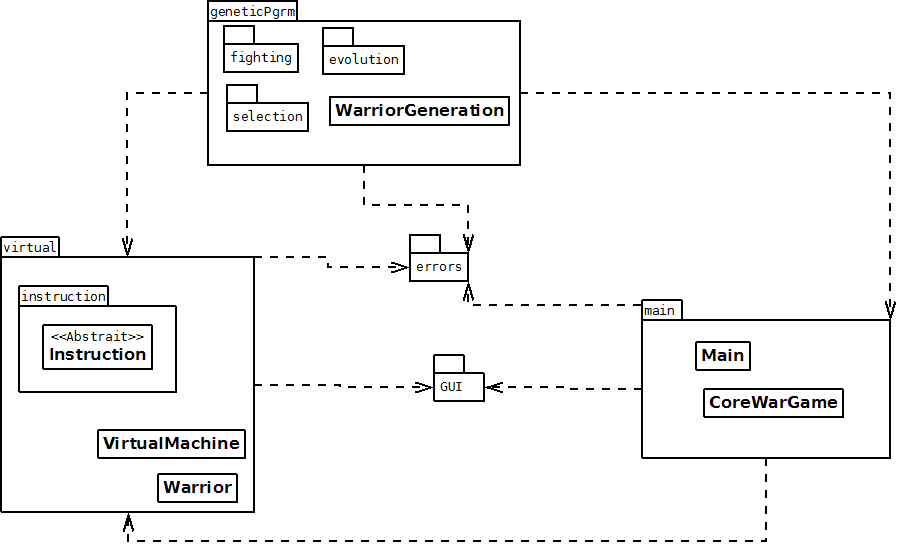
\includegraphics[scale=0.6]{images/diagrammes/archi_gn.png}
    \caption{Architecture générale du projet}
    \label{fig:archiGN}
\end{figure}
\subsection{Architecture de la partie CoreWar}


\begin{figure}[ht]
    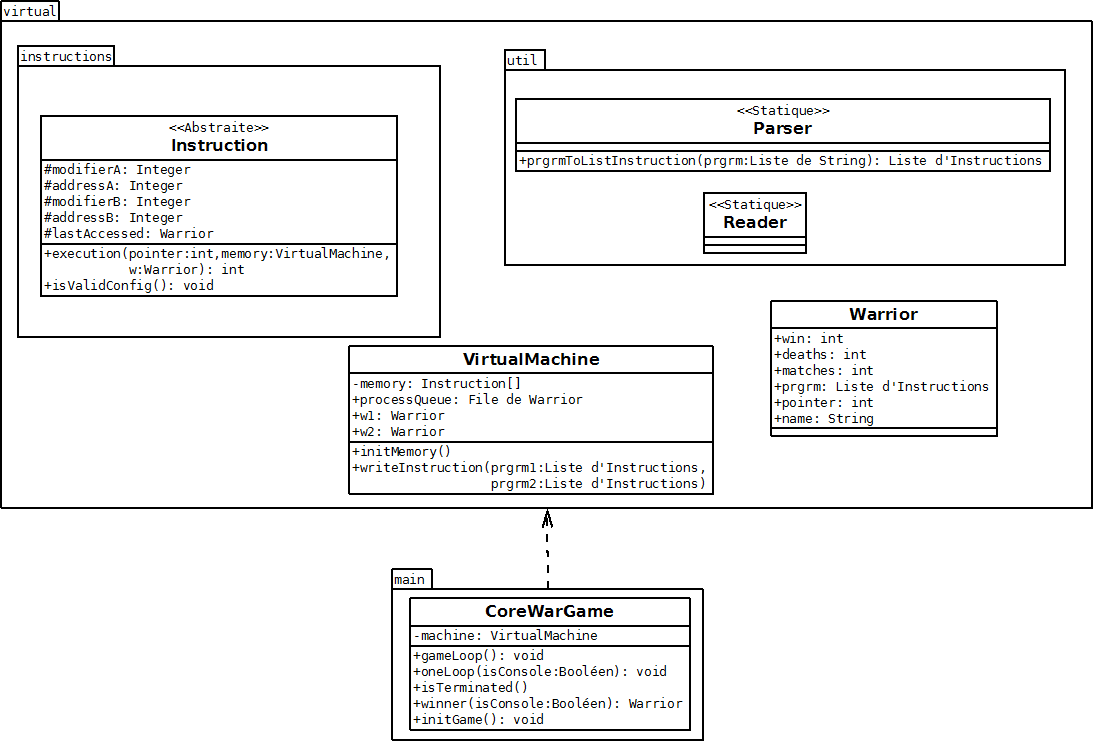
\includegraphics[scale=0.5]{images/diagrammes/partieCW.png}
    \caption{Architecture de la partie CoreWar}
    \label{fig:my_label}
\end{figure}

La partie CoreWar est consistuée de deux packages principaux: \texttt{main} et \texttt{virtual}. Le package \texttt{virtual} comprends deux sous packages: \texttt{instructions} et \texttt{util}. Une seule classe n'a pas été représentée, la classe \texttt{main} du package du même nom, car elle n'est utilisée que pour lancer le logiciel et n'a pas d'intérêt à être représentée ici.

Le package \texttt{util} n'est spécifique au CoreWar qu'avec la classe \texttt{Parser}. La classe \texttt{Reader} est très générique, elle peut lire tout type de fichier qui contient du texte.

La classe \texttt{Parser} est l'objet qui permet de convertir du RedCode pour notre projet. Sa seule fonction est de récupérer un ensemble de chaînes de caractères, des lignes, et de les transformer en objets de type \texttt{Instruction}. C'est une sorte de compilateur, qui peut jeter des exceptions spécifiques à notre projet.(Voir \autoref{sec:errors})

La méthode principale de l'objet \texttt{Parser} est \texttt{prgrmToListInstruction} (\autoref{subsec:conversion}). Cette classe possède d'autres méthodes pour fragmenter la vérification et la conversion d'une ligne, qui pour la plupart ne renvoient rien, sauf des erreurs si il y en a. Enfin, la classe \texttt{Parser} possède des attributs statiques qui représentent les éléments existants dans le RedCode que nous avons implémenté dans notre projet. 

Le package \texttt{instructions} contient toutes les instructions que nous avons implémentées, sous forme de classes. Toutes ces classes héritent de la classe abstraite \texttt{Instruction}. Cette classe n'est pas vouée à être instanciée car cela n'a pas de sens d'être juste une "instruction", sans précision. En revanche, il est beaucoup plus logique de considérer qu'une ligne de RedCode est à la fois une instruction et à la fois un MOV par exemple.

La classe \texttt{Instruction} est codée selon le schéma \autoref{lineRed}. Si une instruction n'utilise que deux champs, les deux autres sont initialisés à \texttt{null} pour éviter toute ambiguïté. Le dernier attribut est plus particulier, il permet de signifier à qui "appartient" l'instruction sous entendu quel est le dernier Warrior a avoir exécuté cet instruction. Cet attribut est considéré si il faut compter le nombre de cases de la mémoire afin de déterminer un gagnant. La classe \texttt{Instruction} possède deux méthodes principales. La méthode \texttt{execution} est la méthode centrale du CoreWar, elle définit comment une instruction se comporte dans la mémoire. Elle doit avoir la connaissance de la mémoire, du pointeur et également du Warrior, pour savoir qui l'exécute. Cette méthode retourne un \texttt{int}, c'est à dire la valeur du pointeur d'instruction après l'exécution. La méthode \texttt{isValidConfig} est appelée à la création de l'objet, afin de vérifier que la méthode \texttt{execution} est capable d'exécuter l'instruction, avec les champs actuels. Nous aurions pu appeler cette méthode dans le constructeur, ce qui n'est pas le cas ici. Un objet \texttt{Instruction} peut être cloné, pour les besoins de notre projet, ce qui se traduit par l'implémentation de l'interface \texttt{Cloneable}, et par deux constructeurs utilisables.

La classe \texttt{VirtualMachine} est la machine utilisée par le CoreWar. Elle possède une mémoire, qui est un tableau primitif d'\texttt{Instruction}, une file de processus, et la connaissance des Warriors qui sont actuellement dans la machine.

Nous avons des accesseurs publics à la mémoire, afin d'éviter d'accéder au tableau directement, mais les deux méthodes principales de \texttt{VirtualMachine} sont \texttt{initMemory} et \texttt{writeInstruction}.

La méthode \texttt{initMemory} permet de "créer" les cases de la mémoire, en insérant dans chaque case du tableau l'instruction \texttt{DAT \#0} manuellement. La méthode \texttt{writeInstruction} va permettre d'écrire les programmes des deux Warriors dans la mémoire, de manière à ce que les deux programmes ne se chevauchent pas. Afin de pouvoir actualiser l'interface graphique après cette écriture, l'appel à cette méthode n'est pas fait dans le constructeur. La machine virtuelle peut exister sans qu'il n'y ait aucun programme à l'intérieur, du moins, un programme qui n'ai pas été inséré par la méthode \texttt{writeInstruction}.

Enfin, la classe \texttt{Warrior} est la matérialisation objet d'un programme RedCode. C'est lui qui sera notamment propriétaire du pointeur d'instruction, il est confondu avec. D'une utilité partielle dans l'exécution d'un CoreWar simple, les attributs de la classe \texttt{Warrior} se révèlent très utiles afin de maintenir les statistiques d'un programme lors du déroulement de l'algorithme génétique.

L'objet assez important du package \texttt{main} est la classe \texttt{CoreWarGame}, qui organise le déroulement du jeu. Il possède les attributs nécessaires vers les objets qui lui sont utiles, notamment la machine virtuelle, et les méthodes pour assurer le déroulement du jeu, de l'initialisation jusqu'à la fin de partie. Nous utilisons cet objet pour l'exécution console autant que pour l'exécution en interface graphique, ce qui implique d'avoir une variable pour contrôler l'affichage en console.

\subsection{Architecture de la partie Interface graphique}

\begin{figure}[h]
    \centering
    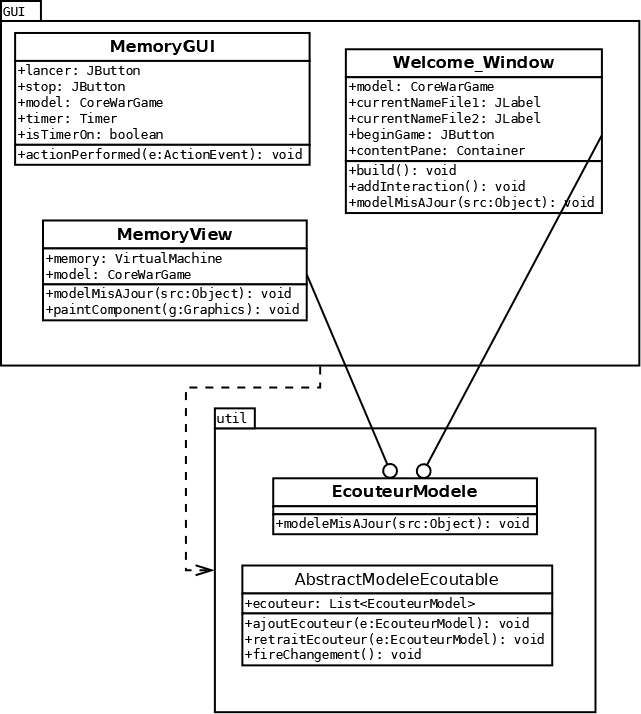
\includegraphics[scale=0.4]{images/diagrammes/archiInterface.png}
    \caption{Architecture de la partie Interface Graphique}
\end{figure}
\vspace{1mm}
L'architecture de l'interface graphique est séparée en deux packages, \texttt{GUI} et \texttt{util}. Le package \texttt{GUI} contient les classes qui permettent l'affichage de la partie graphique, et les classes du package \texttt{util} permettent de gérer les évènements qui mettront à jour l'interface.

Le package \texttt{GUI} possède trois classes. La première est \texttt{Welcome\_Window}. Elle est la première fenêtre que l'on voit lors du lancement du logciel. La classe possède pour attributs un objet \texttt{CoreWarGame}, ainsi que les différents éléments qui composent la fenêtre. Sa méthode \texttt{build} construit la fenêtre en y plaçant les différents éléments. La méthode \texttt{addInteraction} ajoute la possibilité de charger des programmes RedCode et de lancer le jeu. La dernière méthode, \texttt{modelMisAJour}, est hérité de l'interface \texttt{EcouteurModel} et met à jour le nom des champs qui accueil les programmes en modifiant la phrase original par le chemin du fichier.

La classe \texttt{MemoryGUI} permet l'affichage de la fenêtre "principale". Elle a pour but de fournir un support dans lequel dessiner la machine virtuelle ainsi que les boutons permettant d'interagir avec. Sa seul méthode est \texttt{actionPerformed} qui lance le jeu. Cette classe prend une instance de  \texttt{CoreWarGame} en argument, qu'il passera à la classe \texttt{MemoryView}.

\texttt{MemoryView} est la classe qui dessine la représentation de la machine virtuelle. La vue de la mémoire reçoit un objet \texttt{CoreWarGame} en argument qu'elle ajoute à la classe \texttt{AbstractModelEcoutable} pour permettre l'évolution du dessin en fonction de l'évolution du modèle CoreWarGame. Elle en extrait la machine afin de pouvoir récupérer plus facilement les différents attributs de celle-ci lors du dessin. La classe \texttt{MemoryView} possède deux méthodes qui effacent puis redessinent la vue de la machine virtuelle au fil du jeu.

La méthode \texttt{modelMisAJour} fait appel à la méthode \texttt{repaint} de awt.Component qui permet de faire appel à la deuxième méthode,  \texttt{paintComponent}, qui efface et redessine la mémoire selon son état actuel.

Le package \texttt{util} est composé de deux objets. Une interface \texttt{EcouteurModel}, et une classe abstraite nommé \texttt{AbstractModelEcoutable}.

\texttt{AbstractModelEcoutable} possède en attribut une liste d'écouteurs, qui, ici, est le modèle \texttt{CoreWarGame}. Cette classe utilise trois méthodes. \texttt{ajoutEcouteur}, qui ajoute un écouteur à la liste, \texttt{retraitEcouteur}, qui les retire, et \texttt{fireChangement}, qui demande une mise à jour de l'affichage lorsqu'il est appelé.

L'interface \texttt{EcouteurModel} possède une méthode abstraite \texttt{modelMisAJour} qui prend un objet en argument et dont l'exécution change selon l'appel.

\subsection{Architecture de la partie Génération de programme\label{subsec:archiGP}}
\begin{figure}
    \centering
    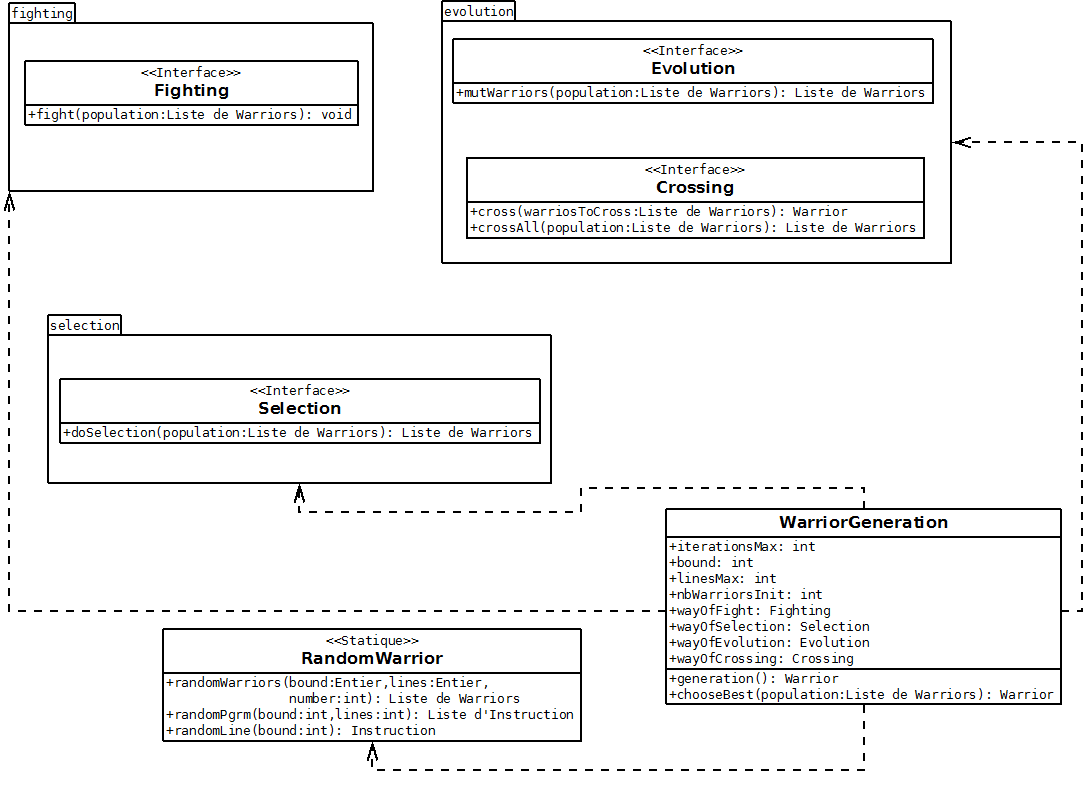
\includegraphics[scale=0.5]{images/diagrammes/partieGP.png}
    \caption{Architecture de la partie Génération de programme}
    \label{fig:partieGP}
\end{figure}
Notre architecture de génération de programme est très modulaire. Elle est séparée en trois sous-packages: \texttt{fighting}, \texttt{selection} et \texttt{evolution}. Dans notre diagramme de classe \autoref{fig:partieGP}, nous n'avons pas précisé les classes implémentant les interfaces indiquées, afin de faciliter la compréhension de l'architecture. Nous n'avons également pas précisé la classe \texttt{Writer} car elle n'est normalement pas spécifique à la génération de programmes, mais si nous mettions cette classe dans le sous-package \texttt{util} du package \texttt{virtual}, ça ne serait pas vraiment sa place non plus. L'idéal aurait été de créer un package \texttt{util} uniquement pour la classe \texttt{Reader} et la classe \texttt{Writer}. Il existe également une classe main spécifique à ce package afin d'instancier la classe \texttt{WarriorGeneration} selon divers paramètres passés par l'utilisateur, elle n'est pas représentée pour les mêmes raisons.


La classe \texttt{RandomWarrior} permet de créer des warriors aléatoirement, ce qui revient à créer aléatoirement des programmes, donc des lignes, comme expliqué à \autoref{algo:randomL}.

La classe \texttt{WarriorGeneration} est la classe principale de ce package, car c'est la classe permettant de générer les programmes performants à partir des outils définis dans les sous-packages. Il reçoit toutes les "options" de configuration: le nombre d'itérations du programme, la limite d'adresse à la génération des programmes, la limite de ligne à la génération des programmes et le nombre de Warriors à générer. De plus, le constructeur attend les outils qui lui permettront de s'exécuter.

Le package \texttt{fighting} est composé de l'interface \texttt{Fighting} qui déclare comment une population de Warriors peut se battre, afin de pouvoir en ressortir un classement. Cela permet de déclarer quel objet peut organiser des combats entre Warriors, ce qui est défini dans la méthode \texttt{fight}, tout en laissant à l'utilisateur le choix des méthodes annexes qui pourrait faciliter son travail. La classe \texttt{WarriorGeneration} n'a besoin que de la méthode \texttt{fight}, peu importe l'objet et le contenu de la méthode. Un exemple de l'implémentation de la méthode \texttt{fight}, dans notre classe \texttt{Tournament}, est \autoref{algo:fight}.

Le package \texttt{selection} est conçu de manière similaire, sauf qu'il concerne cette fois la manière dont les Warriors vont être sélectionnés, afin de ne garder que les meilleurs, selon la sélection opérée. Par défaut, pour faciliter notre implémentation, la classe \texttt{Warrior} est comparable selon le nombre de victoires, mais le choix aurait pu être différent.

Le package \texttt{evolution} est plus fourni, car il contient deux interfaces. L'interface \texttt{Evolution} spécifie comment les Warriors peuvent muter, selon des probabilités laissées à l'utilisateur. Dans notre projet, nous avons créé deux types de classe implémentant cette interface:
\begin{enumerate}
    \item Les classes permettant de réellement modifier les programmes, qui effectuent une action.
    \item Les classes utilisant ces outils, pouvant définir les probabilités d'utilisation et le nombre d'outils utilisés.
\end{enumerate}

Les classes qui permettent d'effectuer les actions sont les outils du second type de classe. Les outils sont encapsulés dans un autre objet afin que du point de vue de la classe \texttt{WarriorGeneration}, il n'y ai qu'une seule méthode à appeler.

La deuxième partie du package \texttt{evolution} est représentée par l'interface \texttt{Crossing} et ses implémentations. Cette interface permet de spécifier comment créer de nouveaux warriors avec la population actuelle. C'est un type d'évolution.
\subsection{Description du package errors}
Le package \texttt{errors} est très simplement constitué. Il est pourvu d'une classe \texttt{CoreWarException}, qui hérite directement de la classe \texttt{Exception} de Java. Nous considérons que les exceptions qui vont être levées doivent obligatoirement avoir un traitement, sinon le reste du programme ne pourrait pas fonctionner. 

Toutes les classes d'exceptions héritent ensuite de \texttt{CoreWarException}, ce qui permet d'attraper spécifiquement les erreurs relatives à notre projet.

Ce package est bien évidemment utile au package \texttt{virtual}, mais également au package \texttt{main}, pour la classe \texttt{CoreWarGame} car l'initialisation de la machine virtuelle peut lever une exception. Enfin, ce package est importé par le package \texttt{geneticPgrm} car la classe \texttt{RandomWarrior} utilise une erreur relative au Parser. Avec cette erreur, nous pouvons définir une mécanique afin de créer des instructions et vérifier en même temps qu'elles sont exécutables. (voir \autoref{algo:randomL})

\section{Cas d'utilisation}
\subsection{Utilisation du CoreWar avec un programme déjà écrit}
Lorsqu'un utilisateur souhaite utiliser le logiciel avec un programme déjà écrit, il doit être attentif à ce que son programme soit écrit sous la forme indiquée \autoref{lineRed}. Il utilisera alors les fonctions permettant l'affrontement de deux programmes RedCode afin de connaître le vainqueur.
\subsection{Génération d'un programme performant}
\begin{figure}
    \centering
    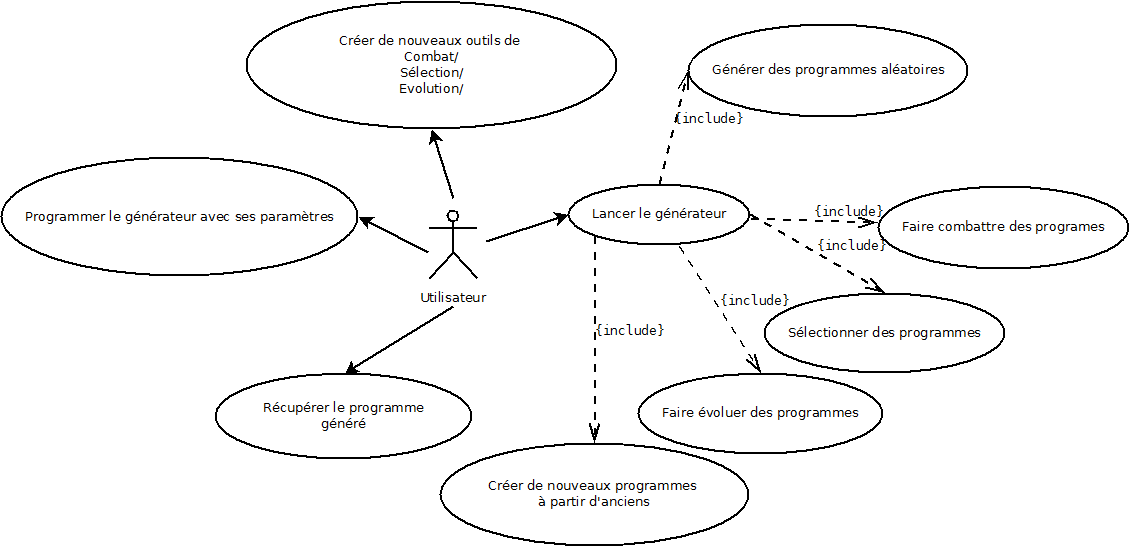
\includegraphics[scale=0.5]{images/diagrammes/casutilisationGP.png}
    \caption{Cas d'utilisation de notre générateur}
    \label{fig:casutilGP}
\end{figure}

Il existe deux types d'utilisateur pour le générateur de programmes performants.

L'utilisateur qui cherche à obtenir un programme performant fonctionnant sur notre CoreWar va utiliser les fonctionnalités lui permettant de programmer le générateur avec ses paramètres, le lancer, et récupérer le programme ainsi généré.

L'utilisateur cherchant plutôt à améliorer ce qui a déjà été fait, ou alors à créer son propre générateur à partir des bases que nous donnons. Il utilisera également la fonctionnalité qui lui permet de créer de nouveaux outils pour le générateur de programme.

\chapter{Expérimentations et usages}

\section{Visuel de l'application}
\subsection{Launcher}
\begin{figure}[H]
    \centering
    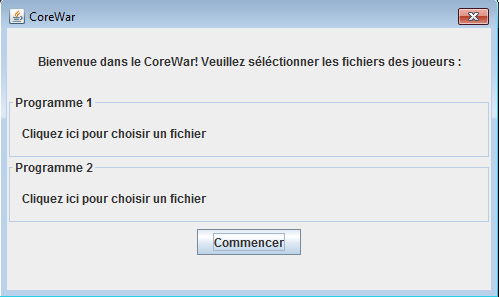
\includegraphics[scale=0.7]{images/visuelauncher.png}
    \caption{La fenêtre d'accueil}
    \label{fig:visulauncher}
\end{figure}
Le launcher de l'interface graphique se présente sous la forme d'une fenêtre dans laquelle nous voyons deux éléments principaux. Les champs qui accueillent le nom des les programmes RedCode, qui invitent l'utilisateur à cliquer dessus afin de sélectionner les programmes, et un bouton "Commencer", qui permet de lancer le jeu une fois les programmes choisis. Si les programmes ne sont pas conformes où qu'il en vient à en manquer un, une fenêtre d'erreur s'affiche, indiquant le problème rencontré.
\subsection{Fenêtre principale}
\begin{figure}
    \centering
    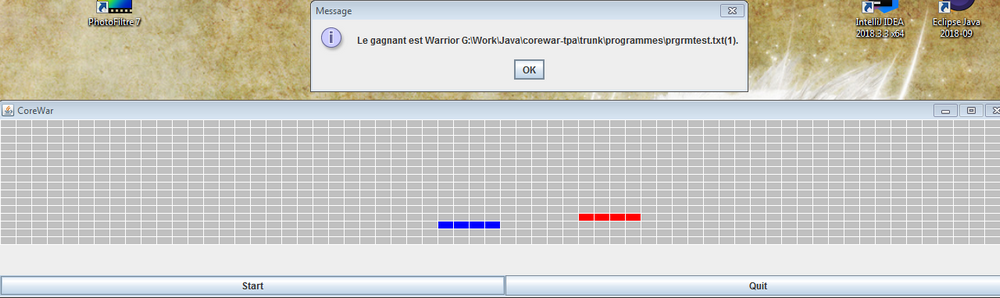
\includegraphics[scale=0.7]{images/visuelinterface2.png}
    \caption{Fenêtre principale}
    \label{fig:visuprincipale}
\end{figure}
Une fois que l'on a cliqué sur le bouton "Commencer", la fenêtre principale s'affiche. Elle présente des lignes de rectangles gris, à l'exception de certain qui sont colorés en bleu et en rouge. Ces rectangles correspondent aux emplacement utilisé par les programmes des joueurs. Les rectangles sont amenés à changer de couleur selon le déroulement de la partie. En dessous, nous trouvons deux boutons, "Start" et "Quit". Le premier sert à lancer la partie, tandis que le second permet de quitter l'application.

\subsection{Visuel en console}
\begin{figure}
    \centering
    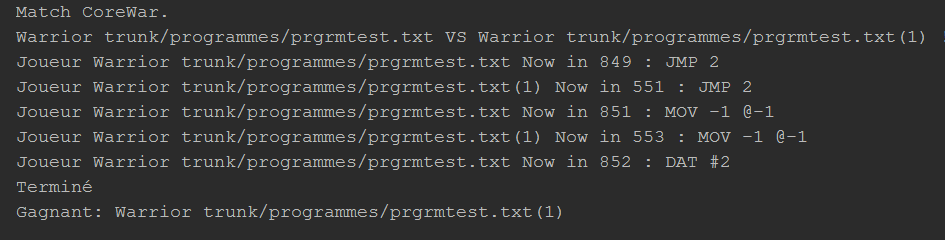
\includegraphics[scale=0.5]{images/visuelconsole.png}
    \caption{Visuel en console}
    \label{fig:consolevisu}
\end{figure}

Le visuel en console est très sobre et précis. Il délimite le début et la fin du combat, et donne le gagnant. En cas de comptage de cases, le nombre de cases de chaque Warrior est affiché, suivi du gagnant.

Pendant l'exécution des programmes, nous avons une ligne pour chaque tour, soit un demi cycle. Voici un schéma pour bien décoder l'affichage. Cet affichage est utilisé pour l'algorithme génétique, bien qu'il soit inutile car les combats sont très rapides et beaucoup de lignes s'accumulent dans la console.

\begin{figure}[H]
    \begin{tikzpicture}
    \node[draw=black] at (0,0) {Joueur Warrior};
    \node[draw=blue] at (4.3,0) {Nom du joueur (chemin du fichier)};
    \node[draw=black] at (8,0) {Now in};
    \node[draw=blue] at (10.8,0) {Position du pointeur};
    \node[draw=blue] at (15,0) {Instruction à cette position};
    \end{tikzpicture}
    \caption{Visuel d'une situation CoreWar sous forme de chaîne}
    \label{fig:visuCoreWar}
\end{figure}

\section{Performances}
Pour les tests de performance avec des temps, nous avons effectués ces tests sur les ordinateurs disponibles dans les salles informatiques via ssh, avec la latence réseau lié à l'accès aux fichiers. Nous avons choisi la microseconde comme unité de temps, car la milliseconde était trop imprécise, mais la nanoseconde donnait des nombres bien trop importants.

Nous signalons que pour chaque expérimentation, nous avons enlevé le résultat du premier test réalisé, car il représentait une anomalie statistique complètement incohérente par rapport à nos résultats. Cela empêchait de lire la courbe des résultats. Nous ne savons pas à quoi est dû cette anomalie.
\subsection{Transformation d'un fichier texte en instructions RedCode exécutables\label{subsec:perfParse}}

Convertir des lignes RedCode en instructions est effectué à chaque lancement du CoreWar, deux fois. De plus, il sera effectué un grand nombre de fois lors de l'utilisation de la méthode \texttt{RandomLine}, sachant que nous n'utilisons pas de Thread pour optimiser les créations de programmes. Cette opération doit prendre le moins de temps possible.

Pour ce faire, nous avons utilisé la classe \texttt{Test\_Parser} afin de tester la méthode \texttt{prgrmToListInstruction}. Nous récupérons le contenu d'un fichier texte de base, qui ne contient qu'une seule ligne, valide. Nous créons un nouveau fichier RedCode, et à chaque itération, nous ajoutons une ligne à ce fichier et nous essayons de le convertir en une liste d'instructions. Cette opération a été répétée 500 fois. Au delà de 500 lignes, nous estimons que le programme n'est pas voué à être lancé, même si il peut rentrer dans la mémoire.

Sur la \autoref{fig:perfParse}, nous remarquons que la courbe générale est quasi linéaire (elle se lève légèrement), malgré quelques pics à certains instants. Entre 300 et 350 lignes, le temps diminue, par rapport à un programme de plus petite taille, ce qui semble montrer que le processeur devait effectuer d'autres tâches pendant une grande partie de nos expérimentations. Néanmoins, le constat reste le même: nous restons en dessous des 1000 microsecondes pour la conversion d'un programme de 500 lignes. Cela correspond à environ 1000 programmes convertis en une seconde. Les deux cas extrêmes, à 100 lignes et 130 lignes, ne semblent pas s'expliquer par la taille du programme, ou par le programme en général, car les opérations effectuées sont linéaires, et la même ligne est présente n fois.

Nous pouvons conclure sur le fait que le Parser reste efficace pour convertir une grande masse d'instructions, et qu'il ne ralentit pas le déroulement du projet.

\begin{figure}[H]
    \centering
    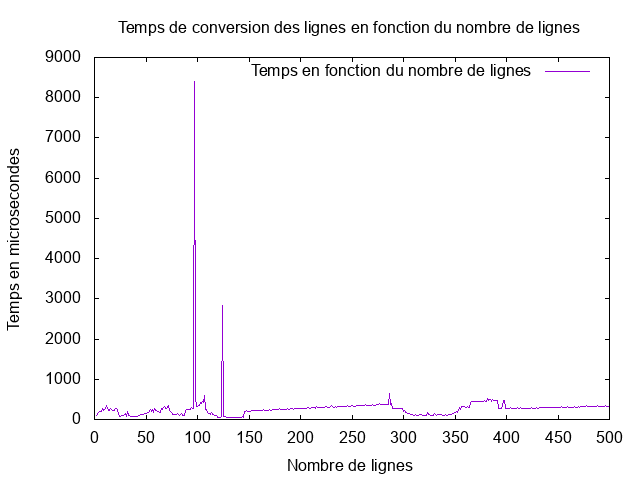
\includegraphics[scale=0.8]{images/graphiques/parserPerf.png}
    \caption{Graphique des performances du \texttt{Parser}}
    \label{fig:perfParse}
\end{figure}

\subsection{Insertion d'ensembles d'instructions dans la mémoire de la machine virtuelle}

L'insertion des programmes dans la machine virtuelle fait appel à un peu d'aléatoire. Nous devons placer deux pointeurs, pour marquer le début des programmes, puis insérer les programmes en respectant la contrainte suivante: les programmes ne peuvent pas se chevaucher. Le premier pointeur est donc placé pseudo-aléatoirement, ce qui se fait en temps constant, mais le deuxième est re-généré aléatoirement tant qu'il ne respecte pas la contrainte. Nous pouvons alors nous demander si il est toujours possible de trouver rapidement un deuxième pointeur qui satisfait cette contrainte. Le temps de placement des programmes va dépendre de la taille des programmes. En effet, plus les programmes sont grands, plus ils vont occuper de placer dans la mémoire, et plus il sera difficile de trouver de l'espace restant pour le second programme. 

Pour tester les performances de notre choix d'algorithme, nous avons repris le principe du test décrit à la \autoref{subsec:perfParse}. Cette fois ci, nous nous sommes limités à des programmes de 350 lignes, car cela fait deux programmes de 350 lignes à insérer la mémoire de la machine, soit 700 lignes.

Nous remarquons que la courbe est dentelée, signe que le temps varie significativement à chaque essai. C'est compréhensible, l'aléatoire pouvant donner plus rapidement ou non des réponses satisfaisantes. Il y a aussi des pics plus ou moins grands, notamment sur un point, aux alentours de 400 en abscisse, où le temps est presque 8 fois plus long qu'en moyenne. Néanmoins, nous pouvons déjà constater qu'insérer jusqu'à 700 lignes ne pose pas de problème à l'algorithme, qui trouve une solution en temps raisonnable. Ce temps raisonnable est majoré par 3000 microsecondes. 

Nous constatons que les pics de lenteur, lié à l'aléatoire, peuvent dépasser 4000 microsecondes, ce qui n'est pas très éloigné du temps raisonnable. Sur les 350 cas engendrés durant ce test, seul un seul a duré 15000 microsecondes, c'est 7 fois plus important que le temps moyen, qui est autour de 2000 microsecondes. Si nous considérons la probabilité d'avoir un tel cas avec nos tests (ce qui n'est pas une bonne façon de faire en général, car il faudrait générer plus de 1000 tests), nous constatons que cette probabilité est de environ 0,003 ce qui est malgré tout très peu.
\\

Nous concluons que malgré l'aléatoire et des pics de lenteur, notre algorithme d'insertion des programmes semble néanmoins efficace, il trouve une solution au problème dans un temps raisonnable et imperceptible au sein du programme.
\begin{figure}
    \centering
    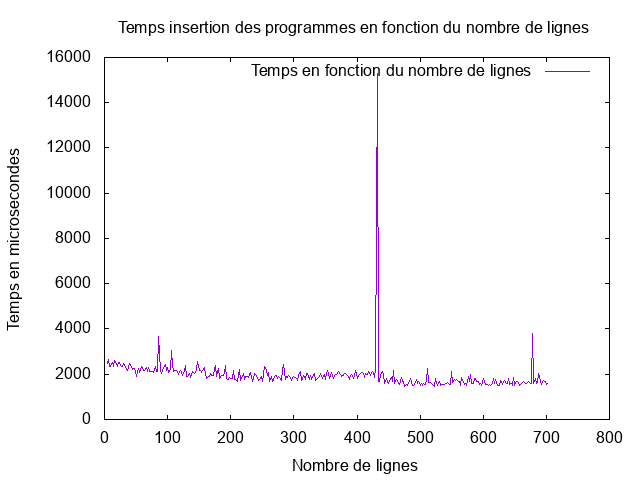
\includegraphics[scale=0.8]{images/graphiques/writePerf.png}
    \caption{Graphique des performances de l'insertion}
    \label{fig:perfInsert}
\end{figure}
\subsection{Création de programmes aléatoires}
\begin{figure}
    \centering
    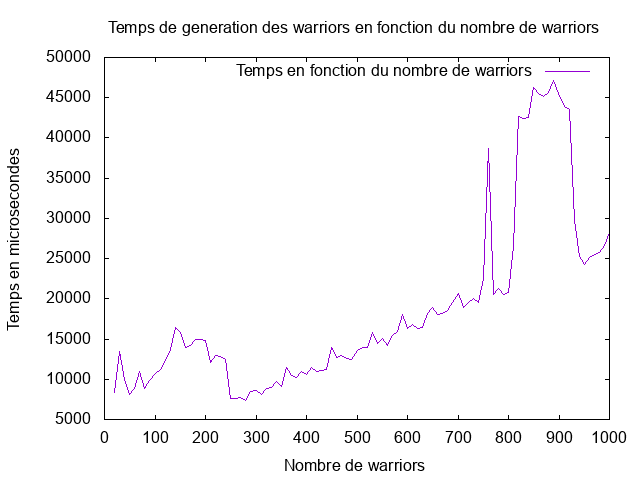
\includegraphics[scale=0.8]{images/graphiques/randomWPerf.png}
    \caption{Graphique des performances de création des programmes aléatoires}
    \label{fig:perfRandomW}
\end{figure}
Notre algorithme génétique repose sur la création de programmes aléatoires, ce qui englobe le fait de créer des instructions mais aussi d'en générer d'autres si elles ne sont pas considérées comme valide. Tout comme l'algorithme précédent, l'aléatoire est impliqué, ce qui nous pousse à nous demander si la création de programmes aléatoires est efficace en temps raisonnable. 

Nous avons effectué le test suivant: nous partons de 10 programmes à générer aléatoirement. La génération aléatoire comprends le choix aléatoire du nombre de lignes du programme, et la création d'une liste de Warriors. Puis nous augmentons le nombre de programmes à générer par pas de 10, jusqu'à 1000. Nous jugeons qu'une population de départ de 1000 est amplement suffisante pour un algorithme génétique bien écrit.

Nous remarquons très logiquement que plus le nombre de programmes à générer augmente, plus le temps augmente également, de façon plus ou moins linéaire. La courbe dessinée entre 300 et 700 warriors montre bien cette linéarité. Cependant, il existe des écarts très importants, pas forcément lié au nombres de warriors à générer. Cela peut être dû au nombre de lignes à générer très important, nombre qui est choisi aléatoire pour chaque programme entre 1 et 10 pour ce test, ou alors au fait que beaucoup d'instructions ont dû être générée (ce qui fait appel au Parser). Mais les pics de lenteurs constatés restent "proportionnels": les pics constatés pour environ 200 warriors sont bien plus petits que les pics pour 800 warriors, ce qui atteste d'une forme de linéarité, si les conditions d'expérimentations étaient parfaites et si l'aléatoire ne créait pas trop d'écart. Pour notre algorithme génétique, nous générons habituellement notre population autour des 200 warriors. 

Sans prendre en compte le pic de lenteur présent sur la courbe, nous pouvons estimer que le temps pour générer cette population va être d'environ 10 000 microsecondes, voire en dessous, ce qui représente un centième de seconde lors de l'exécution. C'est assez énorme, même si imperceptible. Mais en contrepartie, générer 400 warriors, soit le double, prends également 10 000 microsecondes. Le triple, donc 600 warriors, prends 15 000 microsecondes. L'augmentation en temps semble très faible. Enfin, générer 1000 warriors, ce qui semble assez superflu, prends un temps de 27 000 microsecondes, soit environ 3 centième de secondes. Même avec les incertitudes de l'aléatoire, nous pouvons imaginer que nous n'approcherons jamais d'un dixième de seconde pour générer des programmes aléatoires.

La génération de programme aléatoire est très lourde en temps, car nous sommes tout de même à quelques centièmes de seconde, mais cela reste acceptable pour une opération qui forme la base de notre algorithme génétique. Néanmoins, nous pouvons nous demander, par rapport au résultat de notre algorithme génétique, si cette dépense en temps est justifiée ou non. (\autoref{sec:resAG})
\section{Analyse des résultats de l'algorithme génétique\label{sec:resAG}}
Malgré le peu de temps consacré aux tests pour notre projet, nous avons pu néanmoins faire tourner notre algorithme génétique et observer les résultats. Malheureusement, nous n'avons pas pu effectuer de modifications drastiques sur notre algorithme. Nous avons essayé de fournir une première version de l'algorithme génétique tel que nous l'avions conçu, sachant que nous avions très peu de temps pour la conception et l'implémentation. Nos tests se basent sur une population initiale de 200 Warriors et 100 itérations, mais font varier les paramètres, pour voir ce que nous pouvons obtenir.

Première observation: notre algorithme génétique ne fonctionne pas. 

Les programmes qui sortent après 100 itérations ne sont pas du tout performants. Ils meurent très rapidement, alors qu'au sein du déroulement de l'algorithme génétique, certains programmes font de meilleures performances, ne serait-ce qu'en restant sur un ensemble de cases. 

Notre première idée est de penser que c'est à cause de notre méthode de sélection du meilleur programme, à la fin de notre algorithme. Il se base sur les victoires d'un programme, mais cette statistique est biaisée. Certes, plus un programme est performant, plus il gagne, mais plus un programme reste en compétition, plus il a de victoires, ce qui empêche de distinguer le meilleur de celui qui est simplement resté depuis la première étape.

En ayant réinitialisé le compteur de victoire à 0 avant la phase de sélection du meilleur Warrior, l'algorithme sort des programmes qui restent vivants. Ils restent sur un ensemble de cases, plus ou moins grand, jusqu'à que le combat se termine. Ce n'est pas ce que nous attendons d'un programme performant au CoreWar, mais c'est déjà mieux que les précédents résultats.

Nous essayons de réinitialiser le compteur de victoire à 0 pour chaque boucle de l'algorithme. En effet, le raisonnement est le même: un programme ayant moins de victoire aura moins de chance d'être gardé pour l'étape suivante, mais la statistique est biaisée. L'exécution de l'algorithme est plus long, signe que les combats durent plus longtemps, c'est un point positif. Nous obtenons des programmes qui vont occuper plus de cases en mémoire à la fin du CoreWar. De plus, c'est bel et bien la nouvelle génération qui se retrouve en fin d'algorithme, et non pas les warriors du début.

Néanmoins il reste encore beaucoup de problèmes à régler. Déjà, il est possible de trouver un programme qui puisse battre ceux qui sortent de l'algorithme génétique, comme par exemple la seule instruction \textbf{MOV 0 1}, qui "attaque" sans se contenter de rester vivant dans son bout de programme. C'est cette étape que nous ne parvenons pas à franchir. De plus, nous obtenons parfois des programmes très long, car selon notre calcul de la victoire au CoreWar, plus un warrior possède d'instructions, plus il a de chance de gagner, en sachant qu'il possède par défaut les instructions de son propre programme.

Nous n'avons pas beaucoup étudié les evolvers de Warriors déjà existant, et nous n'avons pas étudié en profondeur le principe de l'algorithme génétique, ce qui est une erreur, mais si nous avions donné du temps à ces recherches, nous n'aurions pas pu rendre le projet avec un algorithme qui sort un programme.

Voici quelques idées ressortant de l'étude rapide des evolvers:
\begin{itemize}
    \item Certains evolvers demandent de battre un certain programme pour rester dans la population de départ, lorsqu'il y a génération aléatoire
    \item Le processus de sélection n'utilise pas uniquement le nombre de victoires, mais également le nombre de matchs.
    \item Deux programmes s'affrontent plusieurs fois pour éviter que le placement dans la mémoire joue en leur faveur.
    \item Le score des combats en cas d'atteinte du nombre de cycles maximum est plus nuancé que notre manière de procéder
    \item Certains evolvers donnent le choix entre générer toute la population aléatoirement ou partir d'une population de départ
\end{itemize}

Ces idées pourraient tout à fait être implémentées dans notre projet, si nous avions du temps en plus. Nous ne considérons pas avoir fait de si mauvais choix, mais plutôt ne pas avoir eu le temps de réfléchir et d'étudier de nouvelles idées. Notre faible connaissance de l'algorithme génétique et des evolvers existants n'aurait pas pu permettre un bon algorithme dès le début pour ce projet. 

De plus, certains bugs persistants (\autoref{subsec:bug1} et \autoref{subsec:bug2}) peuvent influencer notre algorithme dans le mauvais sens et causer les mauvais résultats.

Néanmoins, nous considérons que la base de l'algorithme est présente, et que l'algorithme ne produit pas que des programmes stupides, ce qui nous semble un bon début. Nous arrivons à retomber sur l'un des programmes les plus célèbres du CoreWar, le \textbf{MOV 0 1}, à partir d'une génération aléatoire, ou d'autres programmes plus originaux, qui contiennent cette fameuse ligne, ou pas.
\section{Bugs}
Nous allons vous présenter les principaux bugs rencontrés durant le développement. Certains ont pu affecter le projet très fortement, et d'autres n'ont pas pu être résolu à temps. 
\subsection{Lecture de certains champs avec l'objet Parser}
Selon les champs rentrés dans une ligne, par exemple \texttt{\#-10}, le Parser avait des difficultés à extraire le mode d'adressage et l'adresse négative à deux chiffres. 

Le premier bug que nous avions remarqué était celui de l'adresse à deux chiffres. Le Parser prenait le premier chiffre comme un mode d'adressage, et donc relevait une erreur. Le deuxième bug était similaire, mais concernait cette fois le symbole "-" pour les nombres négatifs, confondus avec un mode d'adressage. Le découpage des champs devait être précis et marcher dans tout les cas. A la conception seul un seul cas de figure avait été imaginé.
\subsection{Mise à jour graphique de la machine virtuelle}
À la création de l'interface graphique de la machine virtuelle, les cases se mettaient à jours en colonnes et non en lignes comme voulu.

Ce problème était dû à une inversion de boucle \texttt{for}, où nous créons les colonnes avant les lignes. Nous avons donc échangé l'ordre des deux boucles utilisées afin d'avoir l'affichage souhaité.
\subsection{Obtention d'adresses négatives \label{subsec:bug1}}
Pendant nos exécutions de programmes, notamment pendant l'algorithme génétique, nous avions très souvent des erreurs indiquant que nous souhaitions accéder à une case d'indice négative. Sauf qu'à aucun moment il n'était possible qu'une telle situation arrive, de notre point de vue.

Dans un premier temps, nous avons pensé que c'était l'instruction \emph{SUB} qui faisait apparaître des nombres négatifs. Nous avons donc mis des valeurs absolues pour chaque résultat du \emph{SUB}. Néanmoins, le bug persista, et se déclara dans d'autres instructions. En manque de temps, nous avons décidé de palier à ce bug en ajoutant des valeurs absolues à chaque ligne où le bug se déclenchait.

Finalement, nous avons trouvé la source du bug. Nous utilisons l'opération "\%" (modulo) de Java pour faire nos calculs à l'intérieur de la mémoire, afin de rester entre 0 et 1023 (la taille de la mémoire étant de 1024). Cependant, l'opération modulo de Java n'a pas le comportement espéré: lorsque le nombre à gauche est négatif, le modulo devient négatif, ce qui est mathématiquement incorrect. Une autre fonction existe pour effectuer un vrai modulo: \texttt{Math.floorMod}. Il a fallu donc remplacer chaque modulo par cette fonction, mais cette opération n'a pu être effectué qu'en toute fin de projet à cause du manque de temps critique.
\subsection{Confusion entre les adresses du programme et les adresses après exécution du programme\label{subsec:bug2}}
Notre architecture de la machine virtuelle a un gros défaut: les adresses pendant exécution et les adresses du programme sont confondues. En effet, lors d'une la conversion d'une ligne de RedCode en objet\texttt{Instruction}, les attributs d'adresses sont bien évidemment initialisés avec les valeurs de la ligne. Pendant l'exécution, ces valeurs peuvent changer, ce qui est normal. Ces nouvelles valeurs sont enregistrées en "dur" dans l'objet. Néanmoins, si on réutilise l'instruction (par exemple lors de l'algorithme génétique), ce sont les valeurs actualisées qui sont utilisées, et non pas les valeurs de base du programme. 

C'est une grande faille pour notre projet, car l'algorithme génétique doit être impacté assez sévèrement par ce bug, cela empêche toute stratégie liée à déplacer des blocs de programme par exemple. Pour corriger ce bug, nous pourrions ajouter deux nouveaux attributs à notre classe Instruction, qui représenteraient les adresses pendant exécution. Ainsi, les valeurs d'adresses du programme seraient sauvegardées, et pourraient être rechargées à chaque nouvelle exécution du programme, avec une opération linéaire de ré initialisation sur chaque programme.

Néanmoins, par manque de temps, nous n'avons pas pu corriger ce bug à temps pour le rendu.

\chapter{Conclusion}

\section{Points clés de notre projet}
Utiliser un langage orienté objet pour le CoreWar permet d'avoir une grande modularité dans l'architecture de notre logiciel. Cela permet d'avoir une classe par élément du projet, de mieux les identifier et de faciliter la maintenance du code. Le meilleur exemple vient des instructions. En ayant une classe abstraite pour les gérer, nous pouvons donc ajouter ou retirer une instruction en ajoutant simplement une nouvelle classe lui correspondant. (Même si le Parser ne s'adapterait pas automatiquement)

L'un des points essentiels du projet est de pouvoir récupérer un programme RedCode déjà rédigé pour pouvoir l'appliquer à notre logiciel. L'objet \texttt{Reader} s'en charge conjointement avec l'objet \texttt{Parser}. Ces classes sont importante pour le fonctionnement du logiciel car il est essentiels de pouvoir lire un programme RedCode pour l'exécuter. De plus, notre logiciel joue le rôle d'un compilateur pour RedCode en identifiant les erreurs qui rendent des instructions incompréhensibles ou non exécutables, puis en transformant le RedCode en objets compréhensible de notre logiciel.

Le deuxième point important est l'exécution des programmes qui lui sont donnés. L'utilisation d'une méthode abstraite pour l'exécution de chaque instruction permet de n'appeler que la classe abstraite qui lui est associée et éviter les multiples appels pour vérifier chaque instruction, ce qui permet une plus grande simplicité au niveau de l'implémentation, et de meilleures performances.

Le dernier point remarquable du projet est la création de programmes RedCode selon un algorithme génétique. En se basant sur les lois de l'évolution (Survie du plus fort, mutation aléatoire), le logiciel est capable de créer des programmes performants.

\section{Améliorations techniques envisageable}
Outre les corrections de bugs et les améliorations à apporter sur l'algorithme génétique, nous voulons vous présenter les améliorations possibles de notre projet que nous avons imaginés.
\subsection{Un Parser qui s'adapte en fonction des classes d'instructions présentes}
Notre Parser actuel ne peut gérer que les instructions actuellement écrites. Si l'on souhaite ajouter une nouvelle instruction, il faut modifier le Parser pour qu'il le prennent en compte, sinon l'instruction ne serait pas décodée.

Il faudrait que, dans ce cas, le Parser accède au package \texttt{instruction} et y récupère chaque objet afin de détecter toutes les classes disponibles dans l'immédiat.
\subsection{Configuration possible à partir d'un fichier}
Dans le standard de 1994\cite{standard94} du RedCode, les détails concernant la machine virtuelle sont contenus dans des fichiers de configuration, par exemple la taille de la mémoire ou le nombre de cycles maximum. Nous pourrions bien entendu utiliser ce système pour configurer notre propre machine virtuelle. 

Également, pour certains "evolvers", un fichier de configuration est utilisé pour configurer certains détails comme le nombre d'itérations ou le nombre de Warriors générés, ce que nous pourrions tout à fait faire au lieu de passer nos arguments via la ligne de commande. 
\subsection{Réutiliser un objet VirtualMachine existant}

Lors de l'algorithme génétique, nous chargeons sans cesse de nouvelles instances de \texttt{CoreWarGame}, et donc de nouvelles instances de \texttt{VirtualMachine}. Cela prends du temps et donc fait perdre des performances. 

Puisque nous possédons une machine, avec une mémoire, pourquoi pas la vider et ensuite la recharger avec les nouveaux programmes? Nous utiliserons ainsi une seule instance de \texttt{VirtualMachine}, et par extension une seule instance de \texttt{CoreWarGame} par étape de l'algorithme, au lieu d'en avoir un nombre linéaire, qui dépend de la taille de la population. A savoir ensuite si l'opération de ré initialisation des cases de la mémoire est plus efficace au long terme que de générer de nouvelles instances.
\subsection{Utilisation du multi Thread pour l'algorithme génétique}

Nous n'avons pas eu le temps de nous intéresser aux Threads pour notre projet. Outre la possibilité d'en avoir un afin de gérer notre interface graphique, nous voyons d'autres utilisations utiles du multi-Thread.

L'algorithme génétique peut prendre un certain temps d'exécution, même avec de bons ordinateurs, car le fait de recommencer 100 à 300 fois des opérations linéaires prend beaucoup de temps. Nous pourrions découper certaines étapes, par exemple le croisement des programmes ou le combat des programmes avec des threads, afin d'accélérer ces étapes.

\nocite{*}
\bibliographystyle{plain}
\bibliography{src}

\end{document}
